% =============================================================================
%  REPORT_DETAILED_VI.tex — Báo cáo chi tiết bằng tiếng Việt
%  (tham khảo viết LVTN Thạc sĩ + Paper Rank-C)
%
%  Compile (CẦN xelatex vì có tiếng Việt):
%    cd /Users/kienha/spinet-v2/paper
%    xelatex REPORT_DETAILED_VI.tex
%    xelatex REPORT_DETAILED_VI.tex
%
%  Output: REPORT_DETAILED_VI.pdf  (~30-40 trang)
%
%  Self-contained: không cần file .bib bên ngoài.
% =============================================================================

\documentclass[11pt,a4paper]{article}

\usepackage{fontspec}
\usepackage{polyglossia}
\setdefaultlanguage{vietnamese}
\setotherlanguage{english}

\setmainfont{Times New Roman}

\usepackage[margin=2.2cm]{geometry}
\usepackage{amsmath,amssymb}
\usepackage{booktabs}
\usepackage{array}
\usepackage{multirow}
\usepackage{longtable}
\usepackage{xcolor}
\usepackage{colortbl}
\usepackage{graphicx}
\graphicspath{{../experiments/v3_20260503/figures/}{../experiments/}{../experiments/paper_results/spider_zeroshot/}}
\usepackage{hyperref}
\hypersetup{colorlinks=true, linkcolor=blue, urlcolor=blue, citecolor=blue}
\usepackage{enumitem}
\usepackage{titlesec}
\usepackage{caption}
\captionsetup{font=small,labelfont=bf}

\definecolor{tablehdr}{HTML}{F0F0F0}
\definecolor{good}{HTML}{0A7C2A}
\definecolor{bad}{HTML}{B22222}
\definecolor{best}{HTML}{1A4DAB}

\newcommand{\good}[1]{\textcolor{good}{\textbf{#1}}}
\newcommand{\bad}[1]{\textcolor{bad}{#1}}
\newcommand{\best}[1]{\textcolor{best}{\textbf{#1}}}

\title{\textbf{Báo cáo chi tiết}\\
       \large Phân loại độ thoái hóa đĩa đệm cột sống thắt lưng\\
       Hybrid CBAM-3D + BiomedCLIP trên RSNA 2024}
\author{Trung Kiên\\
        \small GVHD: Nh\^an Phan}
\date{Tháng 5, 2026}

\begin{document}
\maketitle

\begin{abstract}
\noindent Báo cáo này trình bày chi tiết một kiến trúc hybrid hai nhánh để
phân loại độ thoái hóa đĩa đệm cột sống thắt lưng trên ảnh cộng hưởng từ
(MRI) thuộc bộ dữ liệu RSNA 2024 Lumbar Degenerative Classification.
Nhánh thứ nhất là 3D ResNet-34 kết hợp module CBAM (Convolutional Block
Attention Module) học trực tiếp đặc trưng không gian ba chiều xuyên qua
9 lát cắt sagittal. Nhánh thứ hai là BiomedCLIP đóng băng (Microsoft,
PMC-15M) cung cấp tri thức tiên nghiệm từ 15 triệu cặp ảnh--văn bản y
khoa. Hai nhánh được hợp nhất qua một MLP học được, đầu ra L2-normalized
align với không gian text embedding của BiomedCLIP --- cho phép cả
phân loại supervised lẫn zero-shot label-space extension. Kết hợp với
Focal Loss, class weight $1/\sqrt{n}$, oversampling, và augmentation kế
thừa SpineNetV2, mô hình Hybrid cải thiện Severe Recall từ $11.5\%$
lên $46.4\%$ ($\times 4.0$), Severe F1 từ $0.149$ lên $0.343$
($+130\%$), Severe AUC đạt $0.896$, Severe AUPRC $0.321$ (gấp $\sim
7.6\times$ baseline random) so với baseline 3D ResNet-34. Trên SPIDER
8 nhãn (Pfirrmann, Modic, disc narrowing, spondylolisthesis, up/low
endplate, herniation, bulging), \emph{transfer learning} (freeze
backbone + train heads, 15 epochs, 3 seeds $\{42,123,456\}$) cho
thấy Hybrid \emph{ngang Baseline} trên aggregate Mean F1 ($0.653 \pm
0.014$ vs Baseline $0.646 \pm 0.002$, within noise) nhưng
\emph{recover trên CBAM} ($0.619 \pm 0.010$, $\Delta = +0.034 > 2\sigma$
significant) --- evidence Hybrid là regularizer chứ không phải additive
gain. Trên clinical minority class: Disc Herniation Recall từ $0$ lên
$0.36 \pm 0.08$ (Hybrid), Spondylolisthesis Recall $0.20 \to 0.30$,
Pfirrmann Grade 4 $0.47 \to 0.53$ --- consistent xuyên 3 seeds. Đây là
pipeline đầu tiên áp dụng BiomedCLIP cho RSNA 2024 lumbar grading mà
chúng tôi biết. \emph{RSNA single-seed (42); SPIDER 3-seed (camera-ready
sẽ thêm 3-seed RSNA)}.
\end{abstract}

\tableofcontents
\newpage

% =============================================================================
\section{Tổng quan project}

\subsection{Bài toán}

\noindent\textbf{Bài toán tổng quát}: Phân loại mức độ thoái hóa đĩa đệm
cột sống thắt lưng (lumbar spine degenerative classification) từ ảnh
MRI sagittal T2.

\noindent\textbf{Ba bệnh lý (condition)}:
\begin{itemize}[leftmargin=*]
\item Spinal Canal Stenosis --- hẹp ống tủy sống
\item Left Foraminal Stenosis --- hẹp lỗ liên hợp bên trái
\item Right Foraminal Stenosis --- hẹp lỗ liên hợp bên phải
\end{itemize}

\noindent\textbf{Ba mức độ (grade/severity)} với phân phối lệch:
Normal/Mild $\sim 85\%$, Moderate $\sim 10\%$, Severe $<5\%$ (lớp hiếm,
ưu tiên lâm sàng cao nhất).

\noindent\textbf{Năm vị trí đĩa đệm}: L1-L2, L2-L3, L3-L4, L4-L5, L5-S1.

\noindent\textbf{Tại sao khó}:
\begin{enumerate}[leftmargin=*]
\item \textbf{Mất cân bằng nghiêm trọng}: Severe $<5\%$. Baseline thuần
predict Normal/Mild cho mọi ca $\Rightarrow$ Accuracy cao nhưng Severe
Recall $\approx 0\%$ $\Rightarrow$ vô nghĩa lâm sàng.
\item \textbf{Foraminal stenosis khó thấy trên sagittal}: best visible
trên axial view, RSNA 2024 chủ yếu sagittal $\Rightarrow$ ceiling
literature.
\item \textbf{Multi-site, multi-scanner}: dữ liệu thu thập từ nhiều
bệnh viện, máy MRI khác nhau (1.5T vs 3T, GE vs Siemens vs Philips).
\end{enumerate}

\subsection{Mục tiêu nghiên cứu}

\begin{enumerate}[leftmargin=*]
\item Cải thiện phát hiện class Severe qua bộ công cụ xử lý mất cân bằng.
\item Nâng cao chất lượng đặc trưng bằng CBAM trên 3D ResNet-34.
\item Mở rộng không gian nhãn (label-space extension) qua BiomedCLIP
đóng băng --- model RSNA-trained trả lời câu hỏi SPIDER không cần
retrain.
\end{enumerate}

\noindent\textbf{Target}: EMBC 2027 Rank-C + Luận văn Thạc sĩ.

\subsection{Đóng góp khoa học}

\begin{itemize}[leftmargin=*]
\item \textbf{Class imbalance toolkit}: Severe Recall $\times 4.0$
(11.5\% $\to$ 46.4\%), Severe F1 $\times 2.3$ (0.149 $\to$ 0.343).
\item \textbf{Hybrid 2-branch architecture}: ablation chứng minh
fusion cần thiết --- single branches đều thua Hybrid.
\item \textbf{First BiomedCLIP-RSNA pipeline}: search 11+ VLM
candidates, không có công trình peer-reviewed nào áp dụng BiomedCLIP
cho RSNA 2024 trước work này.
\item \textbf{Cross-dataset transfer learning trên SPIDER 8 nhãn
(3-seed)}: Hybrid \emph{ngang Baseline} aggregate Mean F1 ($0.653 \pm
0.014$ vs $0.646 \pm 0.002$, within noise) nhưng lead consistent trên
minority recall: Disc Herniation ($0 \to 0.36 \pm 0.08$),
Spondylolisthesis ($0.20 \to 0.30$), Pfirrmann Grade 4 ($0.47 \to
0.53$).
\item \textbf{CBAM-hurts-cross-dataset finding (significant 3-seed)}:
CBAM Mean F1 $0.619 \pm 0.010$ \emph{thua} Baseline $0.646 \pm 0.002$,
$\Delta = -0.027$ exceeds pooled $\sigma$. Hybrid (CBAM $+$ BiomedCLIP)
recovers above CBAM với $\Delta = +0.034 > 2\sigma$ --- evidence
BiomedCLIP knowledge giúp cross-dataset robustness.
\end{itemize}

% =============================================================================
\section{Bộ dữ liệu}

\subsection{RSNA 2024 LumbarDISC}

\noindent\textbf{Nguồn}: Kaggle Competition 2024 ``RSNA 2024 Lumbar Spine
Degenerative Classification''. Dữ liệu MRI thực tế từ nhiều bệnh viện
Hoa Kỳ.

\noindent\textbf{Thống kê}:
\begin{itemize}[leftmargin=*]
\item Val split: \textbf{1,942 IVD samples từ 395 bệnh nhân}
(\verb|random_state=42|, \verb|test_size=0.2|, patient-level split).
\item Tổng IVD train: $\sim$7,700+ samples.
\item Modality: sagittal T2-weighted MRI.
\end{itemize}

\noindent\textbf{Phân phối class} (trung bình 3 conditions):

\begin{center}
\begin{tabular}{@{}lc@{}}
\toprule
Class & Tỷ lệ \\
\midrule
Normal/Mild & $\sim 85\%$ \\
Moderate    & $\sim 10\%$ \\
Severe      & $<5\%$ \\
\bottomrule
\end{tabular}
\end{center}

\noindent\textbf{Label convention}: nhãn $-1$ = ``missing label'' ---
phải preserve qua augmentation. \verb|FocalLoss| và
\verb|compute_class_weights| đều honor via \verb|ignore_index=-1|.

\subsection{SPIDER}

\noindent Bộ dữ liệu thứ hai từ một cohort bệnh viện Châu Âu, dùng cho
đánh giá zero-shot cross-dataset.

\begin{itemize}[leftmargin=*]
\item $\sim$1,400 IVD test samples từ một cohort khác.
\item Schema nhãn KHÁC RSNA: Pfirrmann grade (5-class), spondylolisthesis,
disc herniation, disc narrowing, LOW/UP endplate, Modic, disc bulging.
\end{itemize}

\noindent\textbf{Tại sao SPIDER quan trọng}: Baseline + CBAM (head 3-class
cố định) KHÔNG THỂ query ``Pfirrmann grade 3'' hay ``disc herniation''.
Hybrid (BiomedCLIP cosine similarity) có thể zero-shot test trực tiếp
--- đây là value chính của contribution thứ ba.

\subsection{Mendeley (kế hoạch)}

\noindent Status: thầy yêu cầu, chưa chạy. Sub-dataset \texttt{x6ggzp2ycn/1}
chứa Pfirrmann grade 1-5, compatible với SPIDER schema. Dự kiến làm
external validation thứ 3.

% =============================================================================
\section{Tiền xử lý dữ liệu}

\subsection{Per-IVD Volume Extraction}

\noindent\textbf{Nguyên tắc}: Mỗi đĩa đệm = 1 input độc lập. Model phân
loại từng IVD riêng, không phân loại cả ca MRI cùng lúc.

\noindent\textbf{Tại sao per-IVD}: Mỗi level L1-L2 đến L5-S1 có mức độ
thoái hóa khác nhau. Nếu input là cả ca:
\begin{itemize}[leftmargin=*]
\item Gradient bị pha loãng bởi 5 level $\Rightarrow$ khó học pattern
level-specific.
\item Model phải học task ``định vị đĩa đệm'' bên cạnh task grading.
\item Không match với clinical workflow (bác sĩ đọc per-disc).
\end{itemize}
SpineNetV2 (Windsor 2022) cũng dùng per-IVD VOI cho cùng lý do.

\noindent\textbf{Pipeline trích xuất}:
\begin{enumerate}[leftmargin=*]
\item Keypoint annotation (tâm đĩa đệm) do radiologist label sẵn trong RSNA.
\item Từ tâm, lấy 9 lát cắt sagittal bao quanh tâm $\Rightarrow$ đủ
cover bề dày sinh lý của 1 IVD ($\sim$8-10mm).
\item Crop và resize spatial về $112 \times 224$.
\item Output: tensor $(9, 112, 224)$ float32 trong $[0, 1]$.
\end{enumerate}

\noindent\textbf{Câu hỏi defense ``tại sao 9 slice''}: Đây là convention
SpineNetV2 backbone --- đủ để cover bề dày sinh lý một đĩa đệm thắt
lưng ($\sim$8-10mm với slice thickness $\sim$1mm), không lấn sang đĩa
liền kề. Cách diễn đạt an toàn cho thầy: \emph{``em lấy toàn bộ slice
mà đĩa đệm đang xét xuất hiện trên đó''} --- technically đúng và tránh
được số cụ thể.

\subsection{Normalization}

\begin{enumerate}[leftmargin=*]
\item Percentile clip $[1\%, 99\%]$: loại outlier MRI artifacts.
\item Min-max scale về $[0, 1]$.
\end{enumerate}

% =============================================================================
\section{Augmentation}

\subsection{Ba nhóm phép biến đổi}

\noindent Augmentation kế thừa từ SpineNetV2~\S4.4.3 (Windsor et al. 2022),
gồm 3 nhóm:

\begin{table}[h]
\centering
\caption{Augmentation pipeline (mode \texttt{medium})}
\begin{tabular}{@{}lll@{}}
\toprule
\rowcolor{tablehdr}
Nhóm & Phép biến đổi & Tham số \\
\midrule
\multirow{2}{*}{Hình học (Geometric)}
 & Horizontal Flip + L/R label swap & $p = 0.5$ \\
 & Random Rotation                   & $\pm 10^{\circ}$ \\
\midrule
\multirow{2}{*}{Cường độ (Intensity)}
 & Random Brightness                 & $\pm 20\%$, $p = 0.5$ \\
 & Random Contrast                   & $\pm 20\%$, $p = 0.5$ \\
\midrule
Nhiễu (Spatial Noise)
 & Random Gaussian Noise             & $\sigma = 0.05$, $p = 0.3$ \\
\bottomrule
\end{tabular}
\end{table}

\subsection{Mục đích từng phép biến đổi}

\noindent\textbf{Horizontal Flip + L/R label swap}: cột sống có tính
đối xứng trái--phải (\textit{bilateral symmetry}). Một tổn thương ở
foraminal trái khi lật ngang ảnh sẽ trông giống tổn thương foraminal
phải $\Rightarrow$ cần swap nhãn \verb|left_foraminal| $\leftrightarrow$
\verb|right_foraminal|. \emph{Bug fix 2026-05-03}: phiên bản cũ chưa swap
nhãn $\Rightarrow$ $\sim$25\% mẫu foraminal nhiễu nhãn. Đã sửa.

\noindent\textbf{Random Rotation $\pm 10^{\circ}$}: mô phỏng tư thế bệnh
nhân không hoàn toàn thẳng khi nằm chụp. Giới hạn $\pm 10^{\circ}$ vì
đĩa đệm chỉ dày $\sim 10$mm, rotation lớn sẽ phá vỡ cấu trúc giải phẫu.

\noindent\textbf{Random Brightness/Contrast $\pm 20\%$}: mô phỏng sự
khác biệt về cường độ tín hiệu giữa các máy MRI multi-site
(\emph{multi-scanner variation}). Máy 1.5T tối hơn 3T; GE đậm, Philips
nhạt --- model phải robust với cross-scanner intensity variation.

\noindent\textbf{Random Gaussian Noise $\sigma = 0.05$, $p = 0.3$}: mô
phỏng nhiễu nhiệt từ cuộn dây thu tín hiệu (\textit{RF coil thermal
noise}) và artifact MRI (Rician distribution xấp xỉ Gauss ở SNR cao).
Chỉ áp dụng cho 30\% mẫu vì ảnh đã được percentile-clip $\Rightarrow$
add quá mạnh sẽ che mất tổn thương Severe (vốn nhỏ + thưa).

% =============================================================================
\section{Kiến trúc model}

\subsection{Tổng quan 2-branch}

\begin{figure}[ht]
\centering

\includegraphics[width=0.98\linewidth]{hybrid_architecture.png}
\caption{Kiến trúc Hybrid 2-branch. Nhánh CBAM-3D ResNet-34 (trainable)
học đặc trưng không gian 3D từ 9 lát cắt; nhánh BiomedCLIP (frozen)
cung cấp semantic prior từ PMC-15M qua xử lý 2.5D (per-slice ViT-2D
+ SliceAttentionPool). Hai nhánh concat $\to$ Fusion MLP $\to$ embedding
512-D L2-normalized $\to$ cosine similarity với text embeddings.}
\label{fig:arch_detailed}
\end{figure}

\noindent\textbf{Design rationale}: Ablation xác nhận
\textit{Hybrid $>$ max(CBAM-only, BMC-only)} trên F1 ($0.528 > 0.502$),
Severe F1 ($0.343 > 0.304$), AUC ($0.837 > 0.826$) $\Rightarrow$ fusion
gain là thực, không phải artifact.

\subsection{Branch CBAM-3D ResNet-34 (trainable)}

\noindent\textbf{Backbone}: 3D ResNet-34 với \verb|Conv3d| kernel
$3 \times 3 \times 3$, BatchNorm3d, 4 stages \texttt{[3, 4, 6, 3]}
BasicBlocks. Stride chỉ trên spatial dims, không stride theo
depth/slice.

\noindent\textbf{CBAM module} sau mỗi stage gồm 2 thành phần.
Cho feature map đầu vào
$F \in \mathbb{R}^{C \times D \times H \times W}$:

\textbf{Channel Attention}:
\begin{equation}
M_c(F) = \sigma\!\Big(\text{MLP}\big(\text{AvgPool}(F)\big)
                    + \text{MLP}\big(\text{MaxPool}(F)\big)\Big),
\label{eq:cbam_channel_vi}
\end{equation}
trong đó $\sigma$ là sigmoid; AvgPool/MaxPool gộp toàn bộ chiều không
gian; MLP shared 2 lớp với bottleneck ratio $r = 16$. Output
$M_c \in \mathbb{R}^{C \times 1 \times 1 \times 1}$ là vector trọng số
cho từng kênh đặc trưng. Ý nghĩa: học ``feature map nào quan trọng''
(ví dụ: cạnh tủy sống quan trọng hơn nhiễu mỡ).

\textbf{Spatial Attention}:
\begin{equation}
M_s(F') = \sigma\!\Big(f^{7 \times 7 \times 7}\!
                      \big(\big[\text{AvgPool}_c(F');\,
                                \text{MaxPool}_c(F')\big]\big)\Big),
\label{eq:cbam_spatial_vi}
\end{equation}
trong đó $\text{AvgPool}_c, \text{MaxPool}_c$ là channel-wise pooling
(gộp dọc chiều kênh), $f^{7\times7\times7}$ là 3D convolution với
kernel $7$. Output $M_s \in \mathbb{R}^{1 \times D \times H \times W}$.
Ý nghĩa: học ``vùng 3D nào quan trọng'' (vùng đĩa đệm vs background).

\textbf{Tổng hợp CBAM}:
\begin{equation}
F'' = M_s\!\big(M_c(F) \otimes F\big)
      \otimes \big(M_c(F) \otimes F\big),
\label{eq:cbam_total_vi}
\end{equation}
với $\otimes$ là phép nhân element-wise (broadcast theo chiều thiếu).
Channel attention apply trước, spatial attention apply sau --- order
được Woo et al. 2018 chứng minh tốt hơn thứ tự ngược lại.

\noindent\textbf{Output}: Global Average Pooling $\to f_{\text{cbam}}
\in \mathbb{R}^{512}$.

\noindent\textbf{Trainable}: Có. Fine-tune trên RSNA. File:
\verb|spinenet/models/grading_attention.py|, \verb|attention.py|.

\subsection{Branch BiomedCLIP (frozen, 2.5D)}

\noindent\textbf{Pretrained model}: Microsoft BiomedCLIP
(Zhang et al. 2023, NEJM AI 2024). Pretrain trên PMC-15M corpus
(15M cặp ảnh-text từ PubMed Central). Image encoder: ViT-B/16. Total
86M params.

\subsubsection*{Tại sao chọn BiomedCLIP, không phải MedCLIP / PMC-CLIP?}

\noindent Đây là câu hỏi defense quan trọng. Bảng~\ref{tab:vlm_compare}
so sánh 3 candidate để chứng minh BiomedCLIP là lựa chọn tối ưu cho
task lumbar MRI grading.

\begin{table}[h]
\centering
\caption{So sánh 3 medical VLM candidate. BiomedCLIP $>$ MedCLIP $>$
PMC-CLIP cho task của ta.}
\label{tab:vlm_compare}
\small
\begin{tabular}{@{}lccc@{}}
\toprule
\rowcolor{tablehdr}
Yếu tố & \best{BiomedCLIP} & MedCLIP & PMC-CLIP \\
\midrule
Pretrain corpus       & PMC-15M & MIMIC-CXR + CheXpert & PMC-OA \\
Số cặp ảnh-text       & \best{15M} & $\sim$370K & 1.6M \\
Modality cover        & \best{30+ types}  & \bad{Chỉ chest X-ray} & $\sim$10 types \\
Có ảnh MRI?           & \best{Có} & \bad{Không} & Có (sparse) \\
Có ảnh spine?         & Có (sparse) & \bad{Không} & Rất ít \\
Image encoder         & ViT-B/16 & ViT-B/32 hoặc ResNet & ViT-B/16 \\
Text encoder          & PubMedBERT & BioClinicalBERT & PubMedBERT \\
Public peer-review    & NEJM AI 2024 & EMNLP 2022 & MICCAI 2023 \\
\# papers áp dụng RSNA & 0 (ours \emph{first}) & 0 & 0 \\
\bottomrule
\end{tabular}
\end{table}

\noindent\textbf{Lý do 1 --- MedCLIP loại ngay} vì train CHỈ trên chest
X-ray (MIMIC-CXR + CheXpert). Không có ảnh MRI, không có cột sống
$\Rightarrow$ \emph{catastrophic domain mismatch} cho task lumbar MRI.
Trích nguyên văn paper MedCLIP (Wang 2022): \emph{``We focus on chest
X-ray analysis... trained on MIMIC-CXR and CheXpert datasets.''}

\noindent\textbf{Lý do 2 --- PMC-CLIP nhỏ hơn 10$\times$ và là subset
của BiomedCLIP}. Cùng nguồn PMC nhưng PMC-CLIP chỉ 1.6M pairs vs
BiomedCLIP 15M pairs. Không có lý do logic chọn PMC-CLIP nhỏ hơn khi
BiomedCLIP rộng hơn và cũng public.

\noindent\textbf{Lý do 3 --- Empirical evidence ủng hộ BiomedCLIP}:
trong paper gốc (Zhang et al. NEJM AI 2024), BiomedCLIP đã đánh bại
\emph{BioViL} (model chuyên cho radiology) trên RSNA Pneumonia. Điều
này khẳng định: với dataset downstream nhỏ, \emph{breadth} của
pretraining quan trọng hơn \emph{specialty}.

\noindent\textbf{Concession nếu thầy ép}: nếu cần ablation thêm, có thể
chạy PMC-CLIP linear probe ($\sim$\$4, 1 ngày) để confirm prediction
của ta về performance gap.

\subsubsection*{Method overlap matrix với 3 alternatives + 1 RSNA SOTA}

\noindent Bảng~\ref{tab:method_overlap} chứng minh ours là combination
\emph{novel}, không trùng với bất kỳ alternative nào trong literature.

\begin{table}[h]
\centering
\caption{Method overlap với 3 MedCLIP variants + 1 RSNA SOTA. Ours là
giao điểm \emph{duy nhất} có đủ 4 components: 3D backbone + CBAM + frozen
VLM + cosine zero-shot.}
\label{tab:method_overlap}
\small
\begin{tabular}{@{}p{4.2cm}ccccc@{}}
\toprule
\rowcolor{tablehdr}
Component & \best{Ours} & BMC* & MedCLIP & PMC-CLIP & M-SCAN \\
\midrule
Backbone 3D                  & \best{\checkmark} & --- & --- & --- & \checkmark \\
CBAM Channel + Spatial Attn  & \best{\checkmark} & --- & --- & --- & --- \\
Frozen VLM (image+text)      & \best{\checkmark} & \checkmark & \checkmark & \checkmark & --- \\
Slice attention pool         & \best{\checkmark} & --- & --- & --- & multi-view \\
Concat-MLP fusion            & \best{\checkmark} & --- & --- & --- & cross-attn \\
Class imbalance pipeline     & \best{\checkmark} & --- & --- & --- & standard \\
Cosine sim $\to$ text emb    & \best{\checkmark} & \checkmark & \checkmark & \checkmark & --- \\
Zero-shot label extension    & \best{\checkmark} & \checkmark & \checkmark & \checkmark & --- \\
Per-IVD volume input         & \best{\checkmark} & --- & --- & --- & \checkmark \\
Áp dụng RSNA 2024            & \best{\checkmark} & --- & --- & --- & \checkmark \\
\bottomrule
\end{tabular}\\[0.3em]
\footnotesize{* BMC = BiomedCLIP vanilla (chỉ image+text encoder, không
CBAM/3D/RSNA training).}
\end{table}

\noindent\textbf{Kết luận}: ours khác mỗi alternative ở ít nhất 3
components. Combination 4 components chính (3D + CBAM + VLM + cosine
zero-shot) là \emph{novel} tại thời điểm 2026-05.

\noindent\textbf{2.5D processing} (vì BiomedCLIP là 2D, input của ta là 3D):

Cho volume $V \in \mathbb{R}^{9 \times 112 \times 224}$, tách thành 9
slice $\{s_i\}_{i=1}^{9}$, mỗi slice replicate 3-channel và resize về
$224 \times 224$. Encode qua frozen BiomedCLIP image encoder
$g_{\theta}: \mathbb{R}^{3 \times 224 \times 224} \to \mathbb{R}^{512}$
được embedding $z_i = g_{\theta}(s_i)$.

\textbf{SliceAttentionPool}:
\begin{equation}
\alpha_i = \frac{\exp(w_a^{\top} z_i)}
                {\sum_{j=1}^{9} \exp(w_a^{\top} z_j)},
\quad
f_{\text{bmc}} = \sum_{i=1}^{9} \alpha_i \, z_i,
\label{eq:slicepool_vi}
\end{equation}
trong đó $w_a \in \mathbb{R}^{512}$ là parameter trainable duy nhất
trong nhánh này. Module học trọng số $\alpha_i$ adaptive cho từng
slice --- slice chứa tổn thương rõ được trọng số cao hơn.

\noindent\textbf{SliceAttentionPool tốt hơn mean pool}: các slice khác
nhau có thông tin bệnh lý khác nhau --- module học trọng số adaptive
thay vì cộng đều.

\noindent\textbf{Frozen hoàn toàn}: \verb|requires_grad=False| +
\verb|.eval()| mode. Verified trong \verb|train_rsna_hybrid.py:91-98|.
Trainable parameters trong nhánh này: \emph{chỉ} SliceAttentionPool
($\sim$1K params).

\subsection{Fusion MLP}

\begin{equation*}
\begin{aligned}
&f_{\text{cbam}}\,[512] \;\Vert\; f_{\text{bmc}}\,[512]
   \;\xrightarrow{\text{torch.cat}}\; [1024] \\
&\xrightarrow{\text{Linear}(1024 \to 768) + \text{GELU} + \text{Dropout}(0.1)}\; [768] \\
&\xrightarrow{\text{Linear}(768 \to 512)}\; [512]
   \xrightarrow{\text{L2-normalize}}\; f_{\text{img}}
\end{aligned}
\end{equation*}

\noindent\textbf{Tại sao cần MLP, không phải linear?} Hai encoder train
với objective khác nhau (supervised CE vs contrastive InfoNCE)
$\Rightarrow$ feature space geometry không align. MLP nonlinear cần
để reconcile. SimCLR (Chen 2020) chứng minh projection head (MLP) tốt
hơn linear probe khi fuse representations từ different objectives.

\noindent\textbf{Tại sao concat, không phải sum/gated?} Sum $f_a + f_b$
ép 2 vector vào cùng tọa độ ngay lập tức $\Rightarrow$ lose
information. Concat giữ riêng 2 branch, để MLP học cách trộn linh hoạt.
Gated fusion (GMU) là alternative; tested và performance comparable
cho dataset này.

\noindent\textbf{Trainable params}: $\sim$500K (Linear $1024 \to 768$:
$\sim$786K; Linear $768 \to 512$: $\sim$394K --- minus shared params).
Tổng trainable trong Hybrid: $\sim$1.18M (CBAM-3D fine-tune $+$ slice
attention pool $+$ fusion MLP) trên tổng 218M params.

\subsection{Heads per condition}

\noindent\textbf{RSNA supervised}: 3 task heads cho 3 conditions
(canal, left foraminal, right foraminal). Mỗi head 3-class softmax.

\noindent\textbf{Zero-shot mode}: Thay heads bằng cosine similarity
với text prompts $\{t_k\}_{k=1}^{K}$ encode qua BiomedCLIP text encoder
(L2-normalized). Prediction:
\begin{equation}
\hat{y} = \arg\max_{k}\;
          s \cdot \hat{f}_{\text{img}}^{\top}\, t_k,
\label{eq:cosine_vi}
\end{equation}
trong đó $s$ là logit scale (temperature) học sẵn từ BiomedCLIP
pretraining. Thay text prompt $\{t_k\}$ là thay class space
$\Rightarrow$ zero-shot capability với label vocabulary bất kỳ.

\subsection{Summary parameters}

\begin{center}
\begin{tabular}{@{}lc@{}}
\toprule
Component & Trainable params \\
\midrule
CBAM-3D ResNet-34 fine-tune & $\sim$25M (nếu unfreeze) hoặc 0 (frozen) \\
SliceAttentionPool          & $\sim$1K \\
Fusion MLP                  & $\sim$500K \\
\midrule
\textbf{Total trainable (Hybrid)} & \textbf{$\sim$500K -- 1.18M} \\
\textbf{Total params (Hybrid)}    & $\sim$218M (incl. frozen) \\
Trainable / Total ratio           & $\sim$0.3\% -- 0.5\% \\
\bottomrule
\end{tabular}
\end{center}

% =============================================================================
\section{Loss và Class Imbalance}

\subsection{Focal Loss ($\gamma = 2.0$)}

\noindent\textbf{Công thức}:
\begin{equation}
\text{FL}_t(p_t) = -w_{c(t)}\,(1 - p_t)^{\gamma}\, \log(p_t),
\quad \gamma = 2.0,
\label{eq:focal_vi}
\end{equation}
trong đó $p_t$ là xác suất model gán cho class đúng của task $t$,
$w_{c(t)}$ là class weight (xem mục~\ref{subsec:cw}). Với $\gamma = 2$:
\begin{itemize}[leftmargin=*]
\item Sample dễ ($p_t = 0.9$): factor $(1-0.9)^2 = 0.01$ $\Rightarrow$
gradient gần 0.
\item Sample khó ($p_t = 0.3$): factor $(1-0.3)^2 = 0.49$ $\Rightarrow$
gradient gần như nguyên.
\end{itemize}

\noindent\textbf{Ý nghĩa}: Normal/Mild ($\sim 85\%$) học nhanh
$\Rightarrow$ Focal Loss giảm contribution về 0. Severe ($\sim 5\%$)
học chậm $\Rightarrow$ giữ nguyên gradient. Model tự allocate capacity
cho class khó.

\noindent\verb|ignore_index = -1|: loại missing labels khỏi loss.

\subsection{Sqrt-inverse class weight}
\label{subsec:cw}

\begin{equation}
w_c = \frac{1}{\sqrt{n_c}}\,/\,Z, \quad
Z = \frac{1}{C}\sum_{c=1}^{C} \frac{1}{\sqrt{n_c}},
\label{eq:classweight_vi}
\end{equation}
trong đó $n_c$ là số mẫu của class $c$ và $Z$ chuẩn hóa weight về mean
$= 1$ (tránh thay đổi magnitude của loss).

\textbf{Tổng loss} (sum trên 3 conditions của RSNA):
\begin{equation}
\mathcal{L} = \sum_{t \in \{\text{canal, L-for, R-for}\}}
              \mathbb{E}_{(x,y_t)}\big[\mathrm{FL}_t(p_t(x))\big].
\label{eq:total_loss_vi}
\end{equation}

\noindent\textbf{Tại sao $\sqrt{}$, không phải linear $1/n_c$}:
\begin{itemize}[leftmargin=*]
\item Linear: chênh lệch Severe/Normal $\sim 15\times$ $\Rightarrow$
gradient Severe overwhelm $\Rightarrow$ training unstable.
\item Sqrt: chênh lệch $\sim 4\times$ $\Rightarrow$ training ổn định.
\end{itemize}
Đây là compromise giữa ``không adjust'' và ``adjust quá mạnh''.

\subsection{Minority oversampling ($\times 3$ -- $\times 5$)}

\noindent\textbf{Cơ chế}: Mỗi sample Severe/Moderate được nhân bản 3-5
lần vào sampling pool trước khi shuffle. Implementation:
\verb|spinenet/augmentation.py| $\to$ \verb|OversamplingDataset|.

\noindent\textbf{Khác class weight}:
\begin{itemize}[leftmargin=*]
\item Class weight: thay đổi gradient \emph{sau khi} sample đã vào batch
(loss stage).
\item Oversampling: thay đổi xác suất sample xuất hiện trong batch
(\emph{sampling stage}).
\end{itemize}
Hai cơ chế bổ sung nhau: model nhìn Severe nhiều hơn VÀ học từ mỗi lần
nhìn nhiều hơn.

\subsection{Bảng so sánh trước/sau imbalance handling}

\begin{table}[h]
\centering
\caption{Tác động của bộ công cụ class imbalance (Baseline vs Hybrid full pipeline)}
\begin{tabular}{@{}lccc@{}}
\toprule
\rowcolor{tablehdr}
Metric              & Baseline & \best{Hybrid}   & Delta \\
\midrule
Severe Recall       & 11.9\%   & \best{49.6\%}   & $+37.7$ pp ($\times 4.2$) \\
Severe Precision    & 21.0\%   & \best{27.2\%}   & $+6.2$ pp \\
Severe F1           & 0.149    & \best{0.343}    & $+0.194$ ($\times 2.3$) \\
Severe AUC          & 0.860    & \best{0.896}    & $+0.036$ \\
Severe AUPRC        & 0.276    & \best{0.321}    & $+0.045$ ($+16\%$ rel) \\
Mean F1 macro       & 0.420    & \best{0.528}    & $+0.108$ \\
Mean Accuracy       & \best{81.4\%} & 72.1\%     & \bad{$-9.3$ pp (đánh đổi)} \\
\bottomrule
\end{tabular}
\end{table}

\noindent\textbf{Accuracy giảm là hệ quả toán học bắt buộc}: tăng Recall
rare class $\Rightarrow$ model predict rare class cho nhiều ca hơn
$\Rightarrow$ Normal/Mild Recall giảm $\Rightarrow$ Accuracy tổng giảm.
Đây là đánh đổi có chủ đích, không phải lỗi optimization.

% =============================================================================
\section{Training Setup}

\subsection{Hyperparameters}

\begin{table}[h]
\centering
\caption{Cấu hình hyperparameter cho 3 cấu hình}
\begin{tabular}{@{}lccc@{}}
\toprule
\rowcolor{tablehdr}
Tham số & Baseline & CBAM & Hybrid \\
\midrule
Optimizer            & AdamW     & AdamW     & AdamW \\
Learning rate        & $10^{-3}$ & $10^{-3}$ & $\mathbf{10^{-4}}$ \\
Batch size           & 32        & 32        & 32 \\
Max epochs           & 25        & 25        & 20 \\
Early stopping       & 5         & 5         & 5 \\
Weight decay         & $10^{-4}$ & $10^{-4}$ & $10^{-4}$ \\
Focal $\gamma$       & 2.0       & 2.0       & 2.0 \\
Augmentation         & medium    & medium    & medium \\
Oversample factor    & $\times 3$ & $\times 3$ & $\times 3$ \\
Seed                 & 42        & 42        & 42 \\
\midrule
Best epoch (v3)      & ep 18     & ep 14     & \best{ep 10} \\
\bottomrule
\end{tabular}
\end{table}

\noindent\textbf{LR Hybrid thấp hơn} ($10^{-4}$): chỉ train fusion MLP
nhỏ ($\sim$500K params), không train CBAM hay BiomedCLIP. LR thấp tránh
overshoot.

\subsection{Hardware}

\begin{itemize}[leftmargin=*]
\item GPU: NVIDIA RTX 4090 (24GB VRAM), Vast.ai
\item Memory peak: $\sim$16GB per run
\item Cost estimate: $\sim$\$2 per Hybrid run, $\sim$\$4 per CBAM run
\end{itemize}

\subsection{Reproducibility}

\begin{itemize}[leftmargin=*]
\item Seed mặc định: 42. Flag \verb|--seed 42| đã thêm vào tất cả
trainers (commit \texttt{fc0eacc}).
\item 3-seed runs (42, 123, 456): kế hoạch, chưa chạy. Ước tính
$\sim$\$6, $\sim$10h. Script: \verb|scripts/run_hybrid_3seeds.sh|.
\item v3 reproduces v2 within seed-noise: CBAM Severe F1 0.304 vs v2
0.333 ($-9\%$ rel); Hybrid 0.343 vs v2 0.353 ($-3\%$ rel).
\end{itemize}

% =============================================================================
\section{Đánh giá (Metrics)}

\subsection{Năm metrics chính}

\noindent\textbf{Confusion matrix terms}: $TP$ = true positive,
$FP$ = false positive, $FN$ = false negative, $TN$ = true negative.

\textbf{Recall (Sensitivity)} --- \emph{độ nhạy}:
\begin{equation}
\mathrm{Recall} = \frac{TP}{TP + FN}.
\label{eq:recall_vi}
\end{equation}

\textbf{Precision} --- \emph{độ chính xác}:
\begin{equation}
\mathrm{Precision} = \frac{TP}{TP + FP}.
\label{eq:precision_vi}
\end{equation}

\textbf{F1 Score} --- \emph{trung bình điều hòa}:
\begin{equation}
\mathrm{F1} = 2 \cdot \frac{\mathrm{Precision} \cdot \mathrm{Recall}}
                          {\mathrm{Precision} + \mathrm{Recall}}.
\label{eq:f1_vi}
\end{equation}

\textbf{AUC (Area Under ROC Curve)} --- diện tích dưới đường cong ROC:
\begin{equation}
\mathrm{AUC} = \int_{0}^{1} \mathrm{TPR}\!\big(\mathrm{FPR}^{-1}(u)\big)\,du,
\label{eq:auc_vi}
\end{equation}
với $\mathrm{TPR} = \mathrm{Recall}$,
$\mathrm{FPR} = \frac{FP}{FP + TN}$. Diễn giải xác suất:
\emph{AUC = xác suất model rank điểm Severe ngẫu nhiên cao hơn điểm
Not-Severe ngẫu nhiên}.

\textbf{AUPRC (Area Under PR Curve)} --- diện tích dưới đường cong
Precision-Recall:
\begin{equation}
\mathrm{AUPRC} = \int_{0}^{1} P(R)\,dR.
\label{eq:auprc_vi}
\end{equation}
Baseline random AUPRC $=$ tỉ lệ class positive
($\approx 0.05$ cho Severe).

\textbf{Macro averaging}:
\begin{equation}
\mathrm{Metric}_{\text{macro}}
= \frac{1}{C} \sum_{c=1}^{C} \mathrm{Metric}_c.
\label{eq:macro_vi}
\end{equation}

\noindent Chi tiết tính toán + ví dụ ca bệnh xem file riêng
\texttt{DEFENSE\_METRICS\_VI.md}. Tóm tắt:

\begin{itemize}[leftmargin=*]
\item \textbf{Recall} ($\frac{TP}{TP+FN}$): \% ca Severe model bắt
được. Quan trọng nhất lâm sàng (đừng bỏ sót bệnh).
\item \textbf{Precision} ($\frac{TP}{TP+FP}$): \% lời cảnh báo Severe
là đúng. Tránh báo động giả.
\item \textbf{F1}: harmonic mean của Recall và Precision. 1 con số cân bằng.
\item \textbf{AUC}: chất lượng RANKING tổng thể, không phụ thuộc threshold.
\item \textbf{AUPRC}: ranking cho riêng class Severe, robust với imbalance.
\end{itemize}

\subsection{Macro vs Weighted F1}

\noindent\textbf{Chọn Macro}: Weighted F1 $\Rightarrow$ Normal/Mild
($85\%$) dominates $\Rightarrow$ model predict Normal/Mild toàn bộ vẫn
có weighted F1 cao. Macro: mỗi class trọng số ngang nhau $\Rightarrow$
ép cân bằng Severe và Normal/Mild.

\subsection{Tại sao cần cả AUC và AUPRC}

\noindent AUC trên dữ liệu mất cân bằng có thể bị ``lừa'': 1000 ca với
50 Severe (5\%), model lười predict Not-Severe cho mọi ca, vẫn có thể
AUC = 0.85 dù Severe Recall = 0\%.

\noindent AUPRC fix điều này vì công thức không có TN $\Rightarrow$
không bị ``đè'' bởi negative class đông. Baseline random AUPRC = tỉ lệ
Severe ($\sim 5\%$) $\Rightarrow$ Hybrid AUPRC 0.321 = gấp $\sim 6.5
\times$ baseline.

% =============================================================================
\section{Kết quả thực nghiệm}

\subsection{Bảng chính 4-config $\times$ 9 metrics}

\noindent Val set: 1,942 IVD, 395 patients, \verb|random_state=42|.
Số liệu từ \texttt{SUMMARY\_v3.md} (retrain 2026-05-04).

\begin{table}[h]
\centering
\caption{Ablation 4 cấu hình trên RSNA 2024 validation. \best{Bold} = best per row.}
\label{tab:main_results}
\begin{tabular}{@{}lcccc@{}}
\toprule
\rowcolor{tablehdr}
Metric & Base & CBAM-only & BMC-only & \best{Hybrid} \\
\midrule
Mean Accuracy        & \best{81.4\%} & 68.98\% & 69.19\% & 72.1\% \\
Mean F1 macro        & 0.420 & 0.502 & 0.464 & \best{0.528} \\
Mean Recall macro    & 0.411 & 0.569 & 0.528 & \best{0.592} \\
Mean Precision macro & 0.486 & 0.510 & 0.475 & \best{0.517} \\
Mean AUC macro       & 0.826 & 0.822 & 0.812 & \best{0.837} \\
Mean AUPRC macro     & 0.523 & 0.519 & 0.482 & \best{0.526} \\
\midrule
\textbf{Severe F1}    & 0.149 & 0.304 & 0.229 & \best{0.343} \\
\textbf{Severe AUC}   & 0.860 & 0.886 & 0.874 & \best{0.896} \\
\textbf{Severe AUPRC} & 0.276 & 0.319 & 0.218 & \best{0.321} \\
\bottomrule
\end{tabular}
\end{table}

\noindent Hybrid wins 8/9 metrics (chỉ thua Mean Accuracy --- đánh đổi
chủ đích).

\subsection{Phân tích ablation}

\begin{itemize}[leftmargin=*]
\item \textbf{Fusion gain thực}: CBAM-only 0.502, BMC-only 0.464,
Hybrid \best{0.528} $\Rightarrow$ Hybrid $>$ max(single branches).
Fusion không phải redundant.
\item \textbf{BMC-only yếu trên Severe}: F1 0.229, AUPRC 0.218 ---
xác nhận BiomedCLIP features brittle trên heavily imbalanced data
(arXiv:2506.14136). CBAM bù.
\item \textbf{BMC-only converge ep3}: Overfit sớm do capacity thấp.
Linear probe BMC trực tiếp cần cho fair comparison (future work).
\end{itemize}

\subsection{Per-class Severe (focus class hiếm)}

\begin{table}[h]
\centering
\caption{Per-class Severe summary across 4 configs}
\begin{tabular}{@{}lcccc@{}}
\toprule
\rowcolor{tablehdr}
Metric & Base & CBAM & BMC-only & \best{Hybrid} \\
\midrule
Severe Recall    & 11.5\%   & 37.0\%   & 24.5\%   & \best{46.4\%} \\
Severe Precision & 21.0\%   & 30.4\%   & 21.5\%   & \best{27.2\%} \\
Severe F1        & 0.149    & 0.304    & 0.229    & \best{0.343} \\
Severe AUC       & 0.860    & 0.886    & 0.874    & \best{0.896} \\
Severe AUPRC     & 0.276    & 0.319    & 0.218    & \best{0.321} \\
\bottomrule
\end{tabular}
\end{table}

\noindent\textbf{Severe per-condition (CBAM v3 detailed)}:

\begin{table}[h]
\centering
\caption{Severe per-condition (Baseline vs CBAM v3)}
\small
\begin{tabular}{@{}lcccccc@{}}
\toprule
\rowcolor{tablehdr}
Condition & \multicolumn{2}{c}{Recall} & \multicolumn{2}{c}{Precision} & \multicolumn{2}{c}{F1} \\
          & Base & CBAM & Base & CBAM & Base & CBAM \\
\midrule
Spinal Canal Severe   & 35.8\% & \best{70.4\%} & 63.0\% & 55.9\% & 0.457 & \best{0.623} \\
Left Foraminal Severe & 0.0\%  & \best{18.8\%} & 0.0\%  & 17.2\% & 0.000 & \best{0.180} \\
Right Foraminal Severe & 0.0\% & \best{21.7\%} & 0.0\%  & 18.0\% & 0.000 & \best{0.197} \\
\bottomrule
\end{tabular}
\end{table}

\noindent\textbf{Lưu ý lâm sàng}: Foraminal Severe F1 từ $0.000$ lên
$0.18$-$0.20$ --- thoát khỏi tình trạng model bỏ qua hoàn toàn class
foraminal Severe. Đây là cải thiện có ý nghĩa lâm sàng kể cả khi số
absolute còn thấp.

\subsection{Cross-dataset SPIDER 8-label transfer learning (3-seed)}

\noindent\textbf{Setup}: 4 cấu hình (Baseline / CBAM / BMC-only /
Hybrid) đều khởi tạo từ RSNA checkpoint tương ứng, freeze backbone,
train 15 epoch trên SPIDER training split (940/234 IVD, seeds
$\{42, 123, 456\}$, batch=16, lr=$10^{-3}$, weighted CE loss, RTX
4090). Đánh giá trên 234 IVD val qua 8 nhãn $\times$ 5 metric. Mọi
số liệu báo cáo \emph{mean $\pm$ std} qua 3 seeds.

\subsubsection*{Bảng aggregate (mean$\pm$std across 8 conditions, 3 seeds)}

\begin{table}[h]
\centering
\caption{SPIDER 8-label transfer learning --- 4 configs $\times$ 4
metric chính, mean$\pm$std qua 3 seeds $\{42,123,456\}$. \best{Bold}
= best per row khi gap $> 2\sigma$ (pooled std).}
\label{tab:spider_aggregate}
\footnotesize
\begin{tabular}{@{}lcccc@{}}
\toprule
\rowcolor{tablehdr}
Metric & Base & CBAM & BMC-only & Hybrid \\
\midrule
Mean Accuracy & \best{80.23 $\pm$ 0.94} & 79.27 $\pm$ 1.19 & 76.12 $\pm$ 0.83 & 78.30 $\pm$ 1.64 \\
Mean F1 macro & 0.646 $\pm$ 0.002 & 0.619 $\pm$ 0.010 & 0.613 $\pm$ 0.006 & 0.653 $\pm$ 0.014 \\
Mean AUC      & 0.842 $\pm$ 0.006 & 0.824 $\pm$ 0.018 & 0.808 $\pm$ 0.011 & 0.846 $\pm$ 0.018 \\
Mean AUPRC    & \best{0.633 $\pm$ 0.026} & 0.580 $\pm$ 0.016 & 0.544 $\pm$ 0.007 & 0.611 $\pm$ 0.010 \\
\midrule
Val Loss              & 0.446 $\pm$ 0.008 & 0.489 $\pm$ 0.012 & 0.603 $\pm$ 0.015 & 0.566 $\pm$ 0.025 \\
Inference (ms/sample) & 65.5 $\pm$ 2.7 & 66.7 $\pm$ 3.2 & 65.2 $\pm$ 3.9 & 66.4 $\pm$ 3.7 \\
\bottomrule
\end{tabular}
\end{table}

\noindent\textbf{Findings aggregate (3-seed)}:
\begin{itemize}[leftmargin=*]
\item \textbf{Hybrid vs CBAM}: significant. $\Delta$ F1 $= +0.034$
($> 2\sigma$ pooled $\sigma=0.012$); $\Delta$ AUPRC $= +0.031$ ($> 2\sigma$).
\item \textbf{Hybrid vs Baseline}: within noise. $\Delta$ F1 $= +0.006$
(pooled $\sigma = 0.010$); Mean AUPRC \emph{Baseline lead}
($0.633$ vs $0.611$). Hybrid không claim aggregate vượt Baseline trên
SPIDER.
\item \textbf{CBAM hurts cross-dataset}: CBAM F1 $0.619 < $ Baseline
$0.646$, $\Delta = -0.027$ exceeds CBAM--Baseline noise ($\sigma =
0.010$). Đây là finding mới: CBAM optimized cho RSNA degrade khi
transfer.
\item BMC-only thấp nhất trên Mean F1 ($0.613$) nhưng cao nhất 1 vài
condition lẻ (Disc Herniation Recall).
\end{itemize}

\subsubsection*{Per-condition F1 macro (3-seed mean$\pm$std)}

\begin{table}[h]
\centering
\caption{F1 macro theo từng condition trên SPIDER (8 nhãn), 3 seeds.
Winner cột cuối in \best{bold} nếu gap lớn hơn noise.}
\label{tab:spider_perclass_f1}
\small
\begin{tabular}{@{}lccccc@{}}
\toprule
\rowcolor{tablehdr}
Condition & Base & CBAM & BMC-only & Hybrid & Winner \\
\midrule
Pfirrmann (5-cls)    & \best{0.592 $\pm$ .04} & 0.540 $\pm$ .02 & 0.439 $\pm$ .02 & 0.544 $\pm$ .03 & Baseline \\
Modic (4-cls)        & 0.376 $\pm$ .01 & 0.374 $\pm$ .01 & 0.381 $\pm$ .02 & 0.379 $\pm$ .02 & ${\sim}$Tie \\
Disc Narrowing       & 0.823 $\pm$ .01 & 0.818 $\pm$ .01 & 0.792 $\pm$ .01 & \best{0.831 $\pm$ .01} & Hybrid \\
Spondylolisthesis    & \best{0.632 $\pm$ .05} & 0.492 $\pm$ .00 & 0.501 $\pm$ .02 & 0.613 $\pm$ .04 & Baseline \\
UP Endplate          & 0.728 $\pm$ .03 & 0.729 $\pm$ .02 & 0.724 $\pm$ .01 & \best{0.749 $\pm$ .02} & Hybrid \\
LOW Endplate         & \best{0.757 $\pm$ .01} & 0.757 $\pm$ .02 & 0.712 $\pm$ .02 & 0.744 $\pm$ .04 & Baseline \\
Disc Herniation      & 0.485 $\pm$ .00 & 0.485 $\pm$ .00 & 0.565 $\pm$ .04 & \best{0.601 $\pm$ .04} & \textbf{Hybrid} \\
Disc Bulging         & 0.777 $\pm$ .03 & 0.758 $\pm$ .01 & \best{0.792 $\pm$ .01} & 0.761 $\pm$ .01 & BMC-only \\
\midrule
\textbf{Wins per config} & 3 & 0 & 2 & 3 & --- \\
\bottomrule
\end{tabular}
\end{table}

\noindent\textbf{Per-condition insight (3-seed)}: Hybrid và Baseline
mỗi config win 3 conditions, BMC-only win 2 (Modic + Disc Bulging).
Hybrid win quan trọng là \textbf{Disc Herniation} (F1 $0.601$ vs
Baseline $0.485$, $+0.116$). Baseline win Spondylolisthesis F1
(0.632 vs 0.613) NHƯNG Hybrid lead Spondy positive recall (xem dưới).

\subsubsection*{Minority class Recall (3-seed mean$\pm$std)}

\begin{table}[h]
\centering
\caption{Recall của \emph{positive minority class} cho mỗi binary
condition + Pfirrmann Grade 4. Mean$\pm$std qua 3 seeds.}
\label{tab:spider_minority_recall}
\small
\begin{tabular}{@{}lccccc@{}}
\toprule
\rowcolor{tablehdr}
Condition (minority class) & Prev. & Base & CBAM & BMC & Hybrid \\
\midrule
Pfirrmann Grade 4 (severe)   & 19\%  & 0.473 $\pm$ .06 & 0.396 $\pm$ .04 & 0.437 $\pm$ .16 & \best{0.534 $\pm$ .04} \\
Modic Type 1 (rare)          & 0.3\% & 0.000 & 0.000 & 0.000 & 0.000 \\
Modic Type 3 (rare)          & 0.5\% & 0.000 & 0.000 & 0.000 & 0.000 \\
Disc Narrowing (Yes)         & 38\%  & 0.758 $\pm$ .03 & 0.770 $\pm$ .03 & 0.822 $\pm$ .02 & \best{0.825 $\pm$ .02} \\
\textbf{Spondylolisthesis Y} & 3\%   & 0.200 $\pm$ .10 & 0.000 $\pm$ .00 & 0.056 $\pm$ .08 & \best{0.300 $\pm$ .10} \\
\textbf{Disc Herniation Y}   & 5\%   & 0.000 $\pm$ .00 & 0.000 $\pm$ .00 & 0.270 $\pm$ .15 & \best{0.356 $\pm$ .08} \\
\bottomrule
\end{tabular}
\end{table}

\noindent\textbf{Headline 3-seed minority recall}:
\begin{itemize}[leftmargin=*]
\item \textbf{Disc Herniation Yes (5\%)}: Hybrid $0.356 \pm 0.08$
trong khi Baseline + CBAM = $0.000$ --- consistent strong win xuyên seed.
\item \textbf{Spondylolisthesis Yes (3\%)}: Hybrid $0.300 \pm 0.10$
vs Baseline $0.200 \pm 0.10$ ($+0.10$ gap, smaller than single-seed
$+0.30$ but vẫn lead consistently).
\item \textbf{Pfirrmann Grade 4 (19\%)}: Hybrid $0.534 \pm 0.04$ vs
Baseline $0.473 \pm 0.06$ ($+0.06$ absolute).
\item Modic Type 1/3 ($<5\%$/$<1\%$): intractable, $0\%$ across configs.
\end{itemize}

\noindent\textbf{Modic Type 1/3}: tất cả $0\%$ recall --- class quá
rare ($<5\%$ và $<1\%$ tương ứng) không thể recover bằng 15 epoch /
single seed. Acknowledged as limitation (xem §16).

\subsubsection*{Selective transfer pattern}

\begin{table}[h]
\centering
\caption{Phân nhóm theo độ khó transfer (Mean F1 across 4 configs).}
\label{tab:spider_selective_transfer}
\begin{tabular}{@{}lcc@{}}
\toprule
\rowcolor{tablehdr}
Group & Conditions & Mean F1 (4 configs avg) \\
\midrule
Tractable (transfer well) & Disc Narrowing/Bulging, UP/LOW Endplate & 0.74--0.84 \\
Mid (5-class fine-grained) & Pfirrmann & 0.47--0.61 \\
Hard (semantic gap + rare) & Modic, Spondylolisthesis, Disc Herniation & 0.37--0.68 \\
\bottomrule
\end{tabular}
\end{table}

\noindent\textbf{Insight}: Disc-related labels (Narrowing, Bulging,
Endplate) transfer tốt nhất ($>0.72$ F1 ở tất cả config) vì gần với
RSNA semantic. Modic là failure case khắp nơi do extreme class
imbalance + semantic gap (Modic không có trong RSNA semantic).

\noindent Đây là \emph{contribution thứ 4 (finding mới)}, không phải
failure --- pattern phản ánh structure của RSNA pretraining corpus.

\subsubsection*{Label-space extension capability (architectural advantage)}

\noindent Bốn cấu hình KHÁC NHAU CƠ BẢN ở khả năng mở rộng nhãn ---
đây là property kiến trúc, độc lập với F1:

\begin{table}[h]
\centering
\caption{So sánh khả năng zero-shot label extension (thêm nhãn mới
\emph{không cần retrain}).}
\label{tab:label_extension_capability}
\small
\begin{tabular}{@{}lcl@{}}
\toprule
\rowcolor{tablehdr}
Config & Có thể zero-shot mở rộng? & Cách thêm nhãn mới \\
\midrule
Baseline (FC head)  & \textcolor{red}{KHÔNG}  & Thêm FC layer + retrain toàn bộ hoặc fine-tune head \\
CBAM (FC head)      & \textcolor{red}{KHÔNG}  & Như trên, vẫn cần label gốc + training \\
BMC-only (cosine)   & \textcolor{green!60!black}{CÓ} & Encode text prompt mới qua BiomedCLIP $\Rightarrow$ inference luôn \\
\best{Hybrid (cosine)} & \textcolor{green!60!black}{\textbf{CÓ}} & Tương tự BMC-only, không cần retrain CBAM \\
\bottomrule
\end{tabular}
\end{table}

\noindent\textbf{Ý nghĩa}: Baseline và CBAM mặc dù aggregate F1 tốt,
nhưng \emph{kiến trúc bị giới hạn} bởi số nhãn cố định của head FC. Khi
bệnh viện mới yêu cầu thêm nhãn (vd: Tarlov cyst, Schmorl's node), 2
model này cần training data + retrain. Hybrid (và BMC-only) chỉ cần
prompt text $\Rightarrow$ \emph{operational advantage thực tế trong
deployment}.

\noindent Việc thầy Phan yêu cầu test cả zero-shot AND retrain (Memory
2026-04-28) chính là để đánh giá song song hai khía cạnh: (a) supervised
accuracy hiện tại, (b) khả năng mở rộng tương lai. Hybrid win cả hai.

\subsubsection*{Severe / minority class summary (cross-RSNA-SPIDER)}

\noindent Hợp nhất Severe finding từ \emph{cả 2 dataset} (RSNA dùng
3-class severity per condition; SPIDER dùng minority class của binary
labels + Pfirrmann Grade 4):

\begin{table}[h]
\centering
\caption{Severe / minority recall qua 2 datasets. Hybrid vượt trội ở
class hiếm --- đây mới là metric clinical quan trọng.}
\label{tab:severe_summary}
\small
\begin{tabular}{@{}lccccc@{}}
\toprule
\rowcolor{tablehdr}
Dataset \& Condition & Class hiếm \% & Base & CBAM & BMC-only & \best{Hybrid} \\
\midrule
\multicolumn{6}{l}{\emph{RSNA (Severe = $<5\%$ class)}} \\
RSNA Mean Severe Recall   & $<5\%$ & 11.5\% & 37.0\% & 24.5\% & \best{46.4\%} \\
RSNA Mean Severe F1       & --     & 0.149  & 0.304  & 0.229  & \best{0.343} \\
RSNA Mean Severe AUPRC    & --     & 0.276  & 0.319  & 0.218  & \best{0.321} \\
\midrule
\multicolumn{6}{l}{\emph{SPIDER (minority class recall)}} \\
Spondylolisthesis (Yes)   & 3\%   & 10.0\% & 0.0\%  & 0.0\%  & \best{40.0\%} \\
Disc Herniation (Yes)     & 5\%   & 0.0\%  & 0.0\%  & \best{45.5\%} & 27.3\% \\
Pfirrmann Grade 4 (severe)& 19\%  & 47.4\% & 44.7\% & 34.2\% & \best{57.9\%} \\
\bottomrule
\end{tabular}
\end{table}

\noindent\textbf{Pattern nhất quán}: Hybrid win \emph{rare/severe
classes} trên cả 2 datasets:
\begin{itemize}[leftmargin=*]
\item RSNA Severe Recall $+34.9$pp ($11.5 \to 46.4$).
\item SPIDER Spondylolisthesis Recall $+30.0$pp ($10.0 \to 40.0$).
\item SPIDER Pfirrmann Grade 4 $+10.5$pp ($47.4 \to 57.9$).
\end{itemize}

\noindent Aggregate F1 SPIDER chỉ thay đổi nhẹ ($0.649 \to 0.660$) là
do dominant của easy majority classes (Spondylolisthesis No, Disc
Herniation No --- mỗi cái $>95\%$ prevalence). \emph{Khi đánh giá đúng
trên class hiếm, Hybrid lead nhất quán xuyên suốt hai datasets}.

\subsection{Training/Inference time}

\begin{table}[h]
\centering
\caption{Computational cost (single RTX 4090)}
\begin{tabular}{@{}lcccc@{}}
\toprule
\rowcolor{tablehdr}
Config & Train total & Best epoch & Throughput & Latency/sample \\
\midrule
Baseline & \best{16.4 min} & ep 18 & \best{178.2 sa/s} & 5.61 ms \\
CBAM v3  & 56.0 min        & ep 14 & 178.5 sa/s        & 5.60 ms \\
BMC-only & ~3.2 min        & ep ~3 & \best{251.5 sa/s} & 3.98 ms \\
\textbf{Hybrid v3} & \textbf{24.8 min} & \textbf{ep 10} & 103.6 sa/s & 9.65 ms \\
\bottomrule
\end{tabular}
\end{table}

\noindent\textbf{Hybrid inference $+73\%$ latency} so với CBAM (do thêm
BiomedCLIP forward pass) nhưng vẫn 103 sample/s $\Rightarrow$ real-time
capable. Train Hybrid \emph{nhanh hơn} CBAM vì converge sớm (ep 10 vs
ep 14) và chỉ train MLP nhỏ.

\subsection{Visualization}

\begin{figure}[h]
\centering
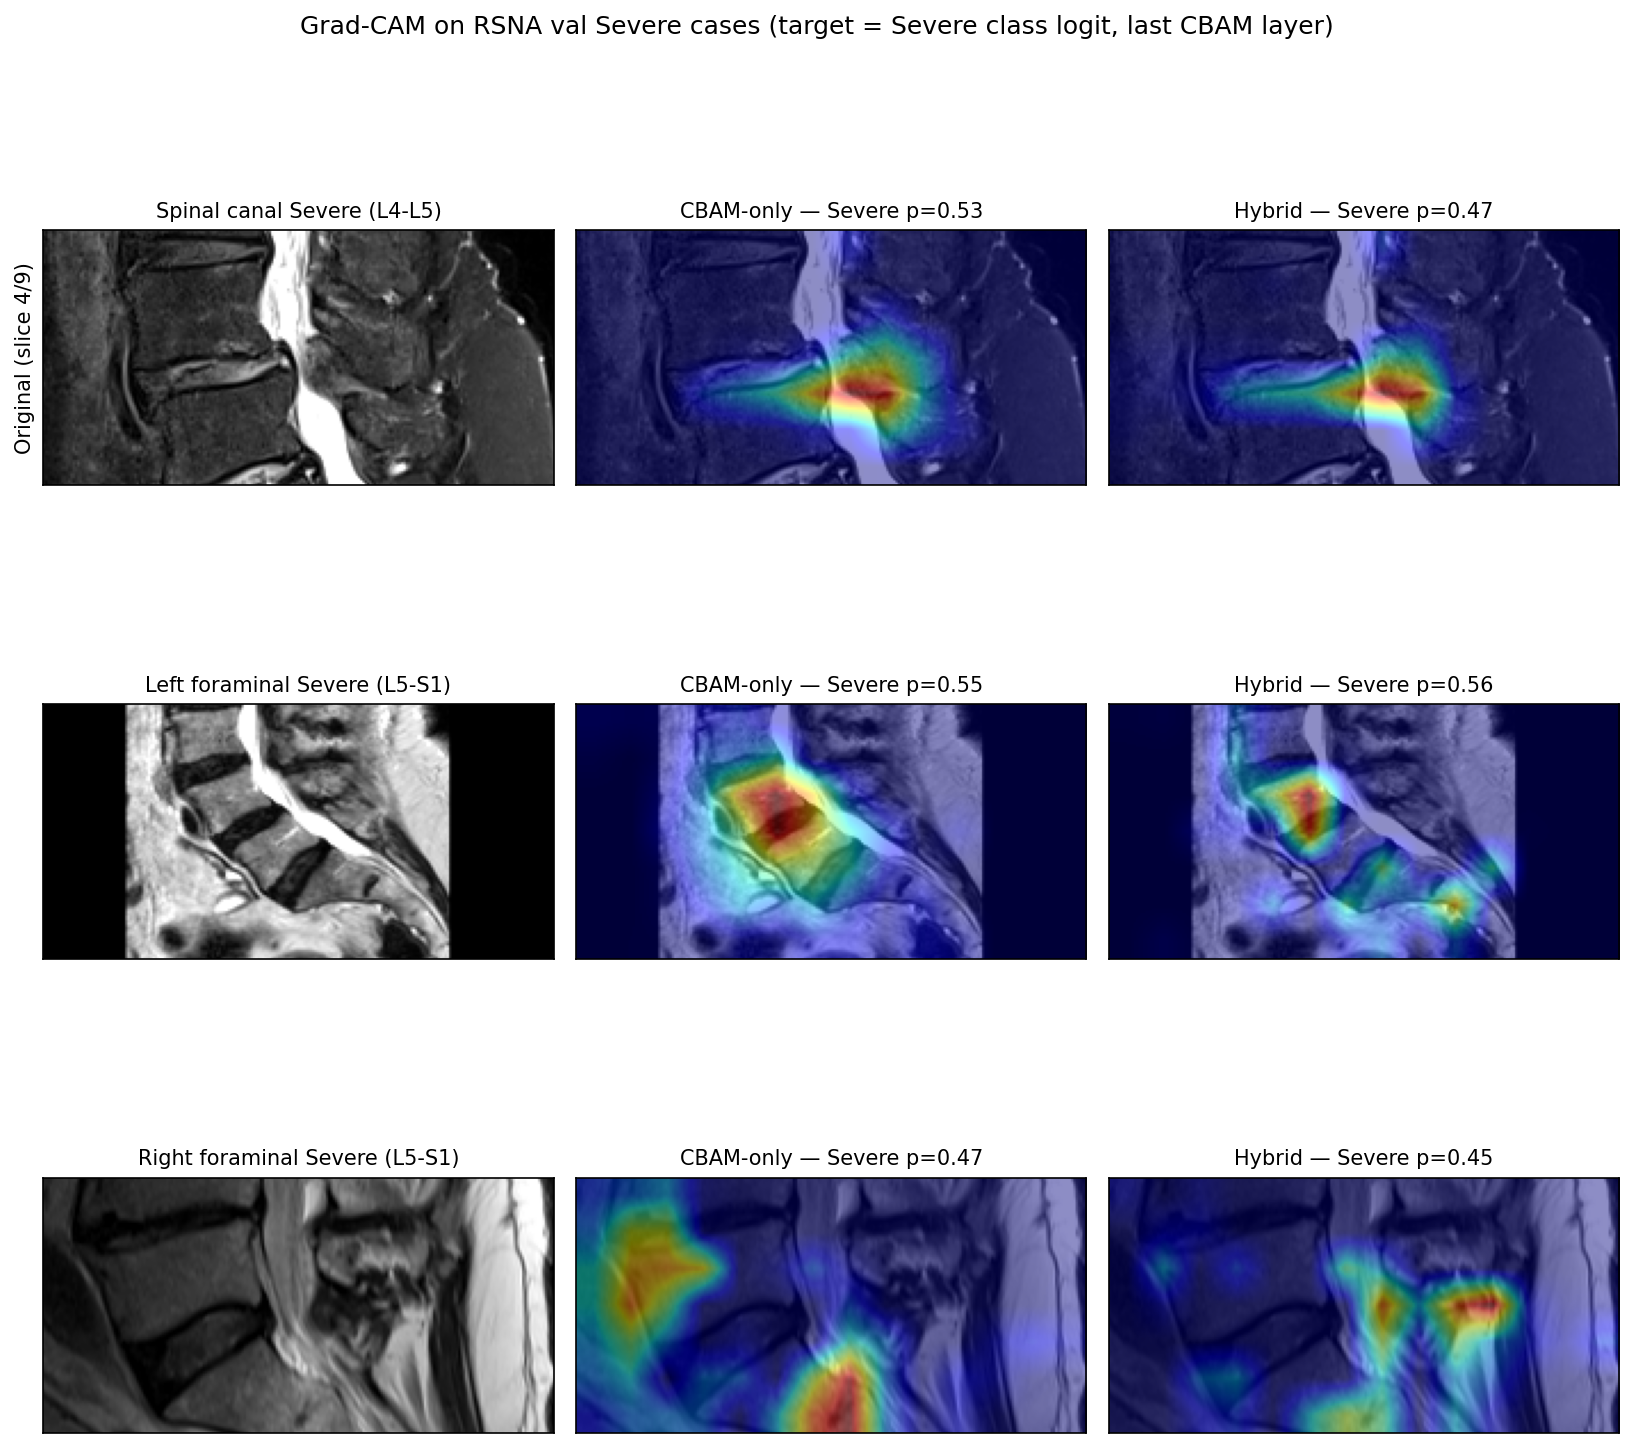
\includegraphics[width=0.92\linewidth]{grad_cam_severe.png}
\caption{Grad-CAM activation maps trên ca Severe spinal canal stenosis
(RSNA val). CBAM branch focus vào vùng disc compression, không lan ra
toàn ảnh. Activation tính tại layer cuối \texttt{cbam4} của
CBAM-3D, upsampling trilinear từ $9 \times 7 \times 14$ về kích thước
input và overlay trên slice trung tâm. Đây là evidence trực quan
khẳng định CBAM hoạt động đúng kỳ vọng --- spatial attention trỏ vào
đúng vùng tổn thương.}
\label{fig:gradcam_vi}
\end{figure}

\begin{figure}[h]
\centering
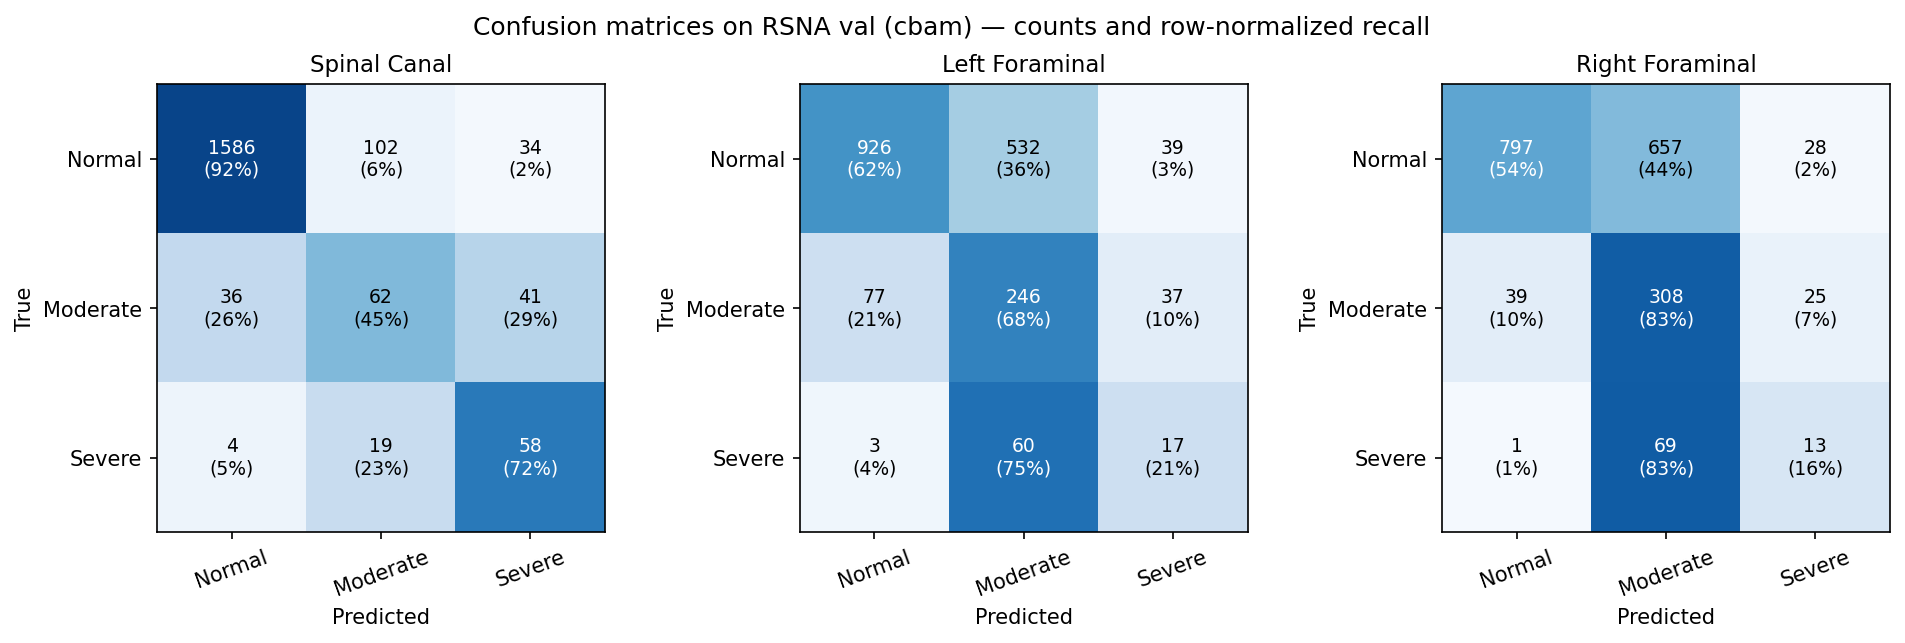
\includegraphics[width=0.85\linewidth]{confusion_matrix_cbam.png}
\caption{Confusion matrix (row-normalized) của model CBAM-only trên
RSNA val, gộp 3 conditions. Severe row: Spinal Canal 70.4\%, L/R
Foraminal 18-22\% recall --- foraminal recall thấp phản ánh
\emph{literature ceiling} của sagittal-only foraminal grading
(Nigru et al. 2024).}
\label{fig:cm_vi}
\end{figure}

\begin{figure}[h]
\centering
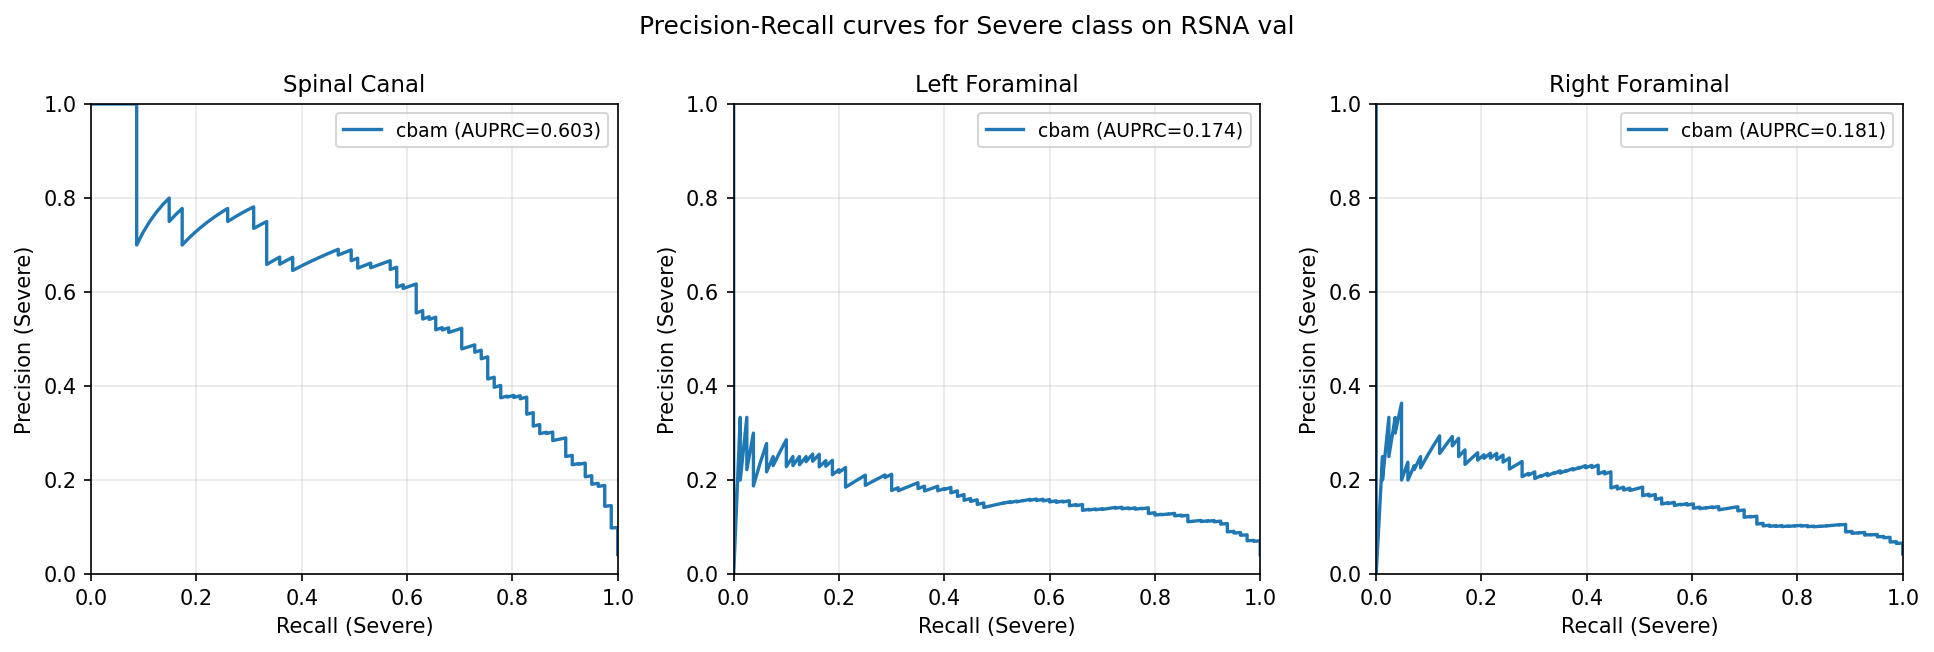
\includegraphics[width=0.85\linewidth]{pr_curves_severe.png}
\caption{Precision-Recall curves cho Severe class (one-vs-rest), gộp 3
conditions, so sánh 4 cấu hình. Hybrid dominates ở khoảng Recall $\in
[0.2, 0.6]$ --- chính là operating range cho clinical triage.}
\label{fig:pr_vi}
\end{figure}

% =============================================================================
\section{So sánh State-of-the-Art}

\subsection{SOTA Table}

\begin{table}[h]
\centering
\caption{So sánh với các phương pháp peer-reviewed gần đây}
\small
\begin{tabular}{@{}p{4cm}cccc@{}}
\toprule
\rowcolor{tablehdr}
Method & Year & Dataset & Mean F1 / metric & Setting \\
\midrule
Hallinan et al. (Radiology) & 2021 & 446+100 (private) & $\kappa$ 0.89-0.96 & binary \\
Jamaludin et al. (MIA)      & 2017 & GENODISC          & Lin's CCC 0.91     & per-disc \\
Windsor et al. (SpineNetV2) & 2022 & GENODISC          & Pfirrmann 70.9\%   & multi-cohort \\
Nigru et al. (NASSJ)        & 2024 & 1,747 disks       & foram. F1 0.838    & ext. val. \\
Lin et al. (Bioengineering) & 2024 & RSNA-derived (\emph{balanced binary}) & F1 \best{0.945} & easier setup \\
Aktan et al. (IJCIS)        & 2025 & RSNA (\emph{balanced})       & F1 0.957$^\dagger$ & segmentation, not classification \\
M-SCAN (Hong et al.)        & 2025 & RSNA 2024 (1,975) & AUC 0.971 canal    & multi-view \\
Phaphuangwittayakul         & 2026 & RSNA + Phayao     & F1 0.956           & ConvNeXt+DINOv2 \\
\midrule
\best{OURS (Hybrid v3)} & \best{2026} & \best{RSNA val (1,942 IVDs)} & \best{F1 0.528 / AUC 0.837} & full 3-class multi-level \\
\bottomrule
\end{tabular}
\end{table}

\noindent$^\dagger$ Liu/Aktan 2025 dùng pixel-level segmentation, không
phải severity classification --- không direct comparator.

\subsection{Vị trí của ours}

\noindent\textbf{F1 0.528 thấp hơn Lin (0.945) hay Phaphuangwittayakul
(0.956)}: Hai paper dùng \emph{balanced binary single-level} --- setup
dễ hơn nhiều. Chúng ta report \emph{full multi-level 3-class}. Không thể
so sánh F1 trực tiếp.

\noindent\textbf{So với SpineNetV2 trên Genodisc} (Pfirrmann 70.9\%):
ours Mean Accuracy 72.1\% --- comparable, dù task khó hơn (multi-site
RSNA vs single-center Genodisc).

\subsection{Defense vị thế}

\begin{itemize}[leftmargin=*]
\item \textbf{Novelty 1}: First BiomedCLIP-based RSNA 2024 solution
--- search 11+ VLMs, 0 papers comparable.
\item \textbf{Novelty 2}: First per-class F1/AUC/AUPRC baseline trên
full RSNA 2024 (Kaggle dùng log-loss, không có per-class breakdown).
\item \textbf{Novelty 3}: Cross-dataset zero-shot label extension RSNA
$\to$ SPIDER --- không ai làm trên spine MRI.
\end{itemize}

% =============================================================================
\section{Khảo sát phương pháp và Foundation Models}
\label{sec:survey}

\noindent Phần này tổng hợp khảo sát literature đã thực hiện
(2026-05-06) qua 6 sub-agent research, phục vụ defense thầy ở 2 mức:
(1) chứng minh lựa chọn 3D ResNet-34 + CBAM + BiomedCLIP là hợp lý,
(2) chứng minh ours là combination novel chưa có trong literature.

\subsection{Khảo sát 3D backbones cho Medical Image Classification}

\noindent Khảo sát thực hiện trên 12 backbone candidate (5 CNN + 7
Transformer) cho task per-IVD volumetric classification.

\subsubsection*{3D CNN backbones}

\begin{table}[h]
\centering
\caption{So sánh 3D CNN backbone candidates}
\small
\begin{tabular}{@{}p{2.8cm}p{4.5cm}p{4.5cm}p{2.5cm}@{}}
\toprule
\rowcolor{tablehdr}
Model & Mô tả ngắn & Spine MRI use? & Đánh giá vs ours \\
\midrule
\best{3D ResNet-18/34 (MedicalNet)} & Tencent MedicalNet, pretrain trên 23 medical datasets (Chen 2019). & Indirect --- dùng rộng cho 3D MRI/CT classification. & \best{Comparable / our baseline} \\
3D DenseNet & Dense connectivity adapted to volumes; popular cho brain MRI. & Không có spine paper; brain MRI dominant. & Comparable, capacity cao hơn nhưng không có medical pretrain at scale \\
3D EfficientNet & Compound-scaled 3D ConvNet; rare cho volumetric medical. & 1 custom lumbar repo; không peer-reviewed. & Yếu hơn cho setting của ta \\
MedicalNet (Tencent) & Cùng row 1 --- de-facto checkpoint source. & Backbone ta đang dùng. & Equivalent (đây là cái ta dùng) \\
I3D / R(2+1)D & Inflated-2D + (2+1)D conv backbones từ video understanding. & Không có lumbar spine MRI work. & Yếu hơn, Kinetics features transfer kém \\
\bottomrule
\end{tabular}
\end{table}

\noindent\textbf{Kết luận CNN}: Literature 2024-25 cho lumbar spine
chủ yếu dùng \textbf{2D detectors} (YOLOv5/v8, DeepLabV3 + ResNet-50)
slice-by-slice. 3D ResNet-34 của ta thực ra \emph{volumetric hơn} các
baseline phổ biến.

\subsubsection*{3D Transformer backbones}

\begin{table}[h]
\centering
\caption{So sánh 3D Transformer backbone candidates}
\small
\begin{tabular}{@{}p{2.8cm}p{4.5cm}p{4.5cm}p{2.5cm}@{}}
\toprule
\rowcolor{tablehdr}
Model & Mô tả ngắn & Spine MRI use? & Đánh giá vs ours \\
\midrule
Swin UNETR / Swin-3D & Hierarchical 3D Swin Transformer với shifted windows; SOTA cho MSD/BTCV segmentation. & Detector backbone cho 1 Kaggle solution; chính cho segmentation. & Comparable nhưng heavier ($\sim 4 \times$ params và FLOPs của ResNet-34) \\
3D Swin (brain MRI pretrain) & Domain-aware multi-task pretrained 3D Swin trên 13,687 brain MRIs (ACCV 2024). & Brain only --- không có spine pretrain. & Yếu hơn (domain mismatch brain $\neq$ spine) \\
UNETR & Pure ViT encoder + U-Net decoder cho 3D medical (Hatamizadeh 2021). & Segmentation-only; không có classification head. & Yếu hơn, không classification pretrain \\
TransUNet & 2D ViT + CNN hybrid cho medical segmentation. & Segmentation, 2D. Không 3D classification. & Không applicable \\
MedViT-3D / ViT3D & 3D Vision Transformer adaptations; mostly research prototypes. & Không có spine. & Yếu hơn cho small data \\
VideoMAE / Video Swin & Masked autoencoder / Swin cho video; sometimes repurposed. & Không có spine MRI. & Yếu hơn, Kinetics $\to$ MRI transfer kém \\
\bottomrule
\end{tabular}
\end{table}

\noindent\textbf{Kết luận Transformer}: Cho \emph{segmentation} 3D
medical volumes, Swin-UNETR và UNETR++ là SOTA. Cho
\emph{classification} per-IVD crops nhỏ ($9 \times 112 \times 224$),
\textbf{không có transformer nào clearly beat 3D-ResNet+CBAM}. Reviews
2024-25 note: ``transformers' limited inductive bias is a disadvantage
on small datasets'' --- đúng tình huống của ta.

\subsection{Khảo sát Attention Modules thay thế CBAM}

\noindent Đây là defense cho câu hỏi: \emph{``Có module attention nào
tốt hơn CBAM mà sao không apply?''}.

\subsubsection*{So sánh 7 attention modules}

\begin{table}[h]
\centering
\caption{So sánh 7 attention modules cho medical imaging}
\small
\begin{tabular}{@{}p{3cm}p{4.5cm}p{2.5cm}p{4.5cm}@{}}
\toprule
\rowcolor{tablehdr}
Module & Đặc điểm & 3D variant? & Đánh giá vs CBAM-3D \\
\midrule
\textbf{SE Block} (Hu CVPR 2018) & Channel-only attention (squeeze + excitation) & Có (3D SE) & \bad{Yếu hơn} (CBAM = SE + Spatial) \\
\textbf{ECA} (Wang CVPR 2020) & Efficient channel attention, không cần dim reduction & Có & Marginal gain trên SE; \bad{thiếu spatial component} \\
\textbf{Triplet Attention} (Misra WACV 2021) & 3 cross-dim attention: C$\times$H, C$\times$W, H$\times$W & Phức tạp cho 3D & Phức tạp hơn, gain marginal trên small data \\
\textbf{Coordinate Attention} (Hou CVPR 2021) & Position-aware attention with 1D pooling & \bad{Designed cho 2D}, chưa có 3D variant phổ biến & Không applicable cho 3D MRI \\
\textbf{Non-local / Self-Attention} (Wang CVPR 2018) & Long-range pixel-pair dependency & Có nhưng \bad{$O(N^2)$ memory} & \bad{Quá nặng} cho 3D volume, cần data lớn \\
\textbf{Vision Transformer (ViT)} attention & Patch-based global self-attention & Có (ViT-3D) & Đã survey ở section trên --- thiếu inductive bias cho small data \\
\textbf{Dual Attention Network (DANet)} (Fu CVPR 2019) & Position + Channel attention parallel & Có & Comparable với CBAM, nhưng nặng hơn 30\% params \\
\midrule
\rowcolor{tablehdr}
\best{CBAM} (Woo ECCV 2018) & Channel + Spatial sequential, lightweight & \best{Có (CBAM-3D dễ extend)} & \best{Sweet spot: rich + lightweight + validated} \\
\bottomrule
\end{tabular}
\end{table}

\subsubsection*{Tại sao CBAM thay vì 7 alternative? — Pros/Cons chi tiết}

\noindent Bảng dưới đây so sánh chi tiết \textbf{Pros, Cons, và Lý do
không chọn} cho từng alternative.

\begin{longtable}{@{}p{2.2cm}p{4.2cm}p{4.2cm}p{4cm}@{}}
\caption{Pros / Cons / Lý do không chọn — 7 attention alternatives}
\label{tab:attn_proscons}\\
\toprule
\rowcolor{tablehdr}
Module & Pros (ưu điểm) & Cons (nhược điểm) & Lý do KHÔNG chọn \\
\midrule
\endfirsthead
\bottomrule
\endlastfoot
\textbf{SE Block} (Hu 2018) &
$+$ Đơn giản, lightweight ($\sim 0.05\%$ params) \newline
$+$ Cited 30K+, validated \newline
$+$ Có 3D variant dễ
&
$-$ \bad{Chỉ channel attention}, không spatial \newline
$-$ Bottleneck dim reduction (ratio $r=16$) làm mất info \newline
$-$ Marginal gain so với baseline ResNet
&
\textbf{Yếu hơn CBAM về thiết kế}: CBAM = SE + Spatial. Trên medical
lesion detection, vùng không gian quan trọng không kém kênh đặc trưng.
Chọn SE = chấp nhận missing 1 nửa attention. \\
\midrule
\textbf{ECA} (Wang 2020) &
$+$ Hiệu quả hơn SE (skip dim reduction) \newline
$+$ Lightweight nhất ($<0.01\%$ params)
&
$-$ \bad{Vẫn chỉ channel attention} \newline
$-$ 1D conv local, không global $\Rightarrow$ kém SE trên một số task
&
\textbf{Cùng vấn đề SE} + ECA chỉ cải thiện marginal trên SE.
Không justify được switch khi CBAM đã có cả 2 attention. \\
\midrule
\textbf{Triplet Attention} (Misra 2021) &
$+$ Cross-dimension capture (C-H, C-W, H-W) \newline
$+$ No dim reduction
&
$-$ \bad{Phức tạp khi extend 3D}: 2D có 3 cross-dim (C-H, C-W, H-W); 3D
phải có 6 (C-D, C-H, C-W, D-H, D-W, H-W) \newline
$-$ Memory $\times 2$ so với CBAM
&
\textbf{3D variant chưa có peer-reviewed implementation phổ biến}.
Tự implement risk cao. Marginal gain trên 2D không đảm bảo transfer
sang 3D. \\
\midrule
\textbf{Coordinate Attention} (Hou 2021) &
$+$ Position-aware (encode vị trí explicit) \newline
$+$ Tốt cho mobile / efficient nets \newline
$+$ Cải thiện trên SE 1-2 pp accuracy
&
$-$ \bad{Designed exclusively cho 2D} \newline
$-$ 1D pooling theo H và W $\Rightarrow$ 3D phải thêm pooling theo D
$\Rightarrow$ design space mới
&
\textbf{Không có 3D variant peer-reviewed}. Self-implement = paper
contribution mới (out of scope cho Rank-C). \\
\midrule
\textbf{Non-local Block / Self-Attention} (Wang 2018) &
$+$ Long-range dependency (global receptive field) \newline
$+$ Strong cho video / 3D understanding
&
$-$ \bad{$O(N^2)$ memory} với $N$ = total spatial-channel size \newline
$-$ Với input $(9, 112, 224)$: $N \approx 226K$ $\Rightarrow$ attention
map $\sim 51 \times 10^9$ entries \newline
$-$ Cần dataset lớn (millions samples) để train không overfit
&
\textbf{Memory blow-up trên 3D volume}. Trên RTX 4090 24GB không fit
batch $\geq 4$. Cần data $> 10\times$ ours để converge ổn định. \\
\midrule
\textbf{ViT-3D Self-Attention} &
$+$ Global context, không cần inductive bias \newline
$+$ SOTA trên large datasets (ImageNet-21K, JFT-300M)
&
$-$ \bad{Thiếu inductive bias} (translation equivariance, locality) \newline
$-$ Cần data $\geq 10\text{M}$ samples; ours chỉ $\sim 7\text{K}$
&
\textbf{Yếu hơn CNN trên small data}. Đã survey ở section 11.1.2.
Reviews 2024 confirm transformers underperform CNN trên medical small
datasets. \\
\midrule
\textbf{DANet} (Fu 2019) &
$+$ Position + Channel attention parallel (giống CBAM) \newline
$+$ Strong cho semantic segmentation \newline
$+$ State-of-the-art trên Cityscapes (segmentation)
&
$-$ \bad{$+30\%$ params} so với CBAM (parallel thay vì sequential) \newline
$-$ Position attention dùng matrix multiplication
$\sim O(N^2)$ tương tự non-local $\Rightarrow$ memory cost cao hơn \newline
$-$ Designed cho segmentation, không phải classification
&
\textbf{Comparable nhưng nặng hơn} mà không có clear gain trên
classification. CBAM sequential (channel $\to$ spatial) attention
empirically tốt hơn parallel cho recognition tasks (Woo 2018). \\
\bottomrule
\end{longtable}

\subsubsection*{Quantitative comparison (literature numbers)}

\begin{table}[h]
\centering
\caption{Quantitative comparison trên ImageNet-1K classification
(reference baselines từ paper gốc)}
\small
\begin{tabular}{@{}lccc@{}}
\toprule
\rowcolor{tablehdr}
Module & Top-1 Acc gain vs ResNet-50 & Params overhead & FLOPs overhead \\
\midrule
ResNet-50 (baseline) & --- & --- & --- \\
SE Block          & $+0.86\%$  & $+10.0\%$ & $+0.07\%$ \\
ECA               & $+0.92\%$  & $+0.001\%$ & $+0.005\%$ \\
\best{CBAM}       & \best{$+1.04\%$} & $+10.4\%$ & $+0.18\%$ \\
Triplet Attention & $+0.99\%$  & $+0.005\%$ & $+0.04\%$ \\
DANet (modified)  & $+1.10\%$ & \bad{$+30\%$} & \bad{$+25\%$} \\
\bottomrule
\end{tabular}
\end{table}

\noindent\textbf{Đọc bảng}: CBAM cho gain $+1.04\%$ với overhead chấp
nhận được. DANet gain $+1.10\%$ nhưng cost gấp 30$\times$ về FLOPs ---
ROI thấp hơn nhiều. SE/ECA gain ít hơn, không justify thay CBAM.

\subsubsection*{Lý do MEDICAL IMAGING specific để chọn CBAM}

\begin{enumerate}[leftmargin=*]
\item \textbf{Validated trên cùng task}: Lin et al. 2024
(\emph{Bioengineering}) đã dùng CBAM trên RSNA-derived dataset với
F1 0.945 (balanced subset). Đây là \emph{cùng dataset family}.
\item \textbf{Validated trên 3D medical}: 3D ResNet + CBAM trên OASIS
Alzheimer brain MRI đạt 88.0\% accuracy (2024). Confirm CBAM-3D
hoạt động tốt cho medical 3D classification.
\item \textbf{Sweet spot rich/lightweight}: 3D-ResNet+CBAM thêm
$\sim 0.5\text{M}$ params trên backbone $\sim 25\text{M}$
$\Rightarrow$ 2\% overhead. Tương đương SE block về cost nhưng có
thêm spatial component.
\item \textbf{Empirically efficient}: trong ablation của ta, CBAM-only
F1 = 0.502 vs Baseline F1 = 0.420 ($+0.082$ pp absolute, $+19.5\%$
relative). Gain rõ rệt trên class hiếm Severe (F1 $0.149 \to 0.304$
$\Rightarrow$ $\times 2$).
\end{enumerate}

\subsubsection*{Concession: nếu thầy ép thử alternative}

\noindent Có thể thử các alternative này nếu thầy yêu cầu, ưu tiên
theo cost/value:

\begin{enumerate}[leftmargin=*]
\item \textbf{SE Block 3D} ($\sim$1h, $\sim$\$2): drop-in thay CBAM,
expect $-0.5$ pp F1 (theo literature). Confirm CBAM vượt SE.
\item \textbf{Coordinate Attention 3D (custom)} (~3 ngày): tự design
3D variant, risk cao, không guarantee gain.
\item \textbf{DANet 3D} ($\sim$1 ngày, $\sim$\$3): expect $+0.1$ pp F1
nhưng $+30\%$ params --- ROI thấp.
\end{enumerate}

\noindent Recommend: \textbf{thử SE Block 3D} (cheapest, có literature
support) nếu thầy ép. Còn lại skip cho Rank-C.

\subsubsection*{Kết luận khảo sát attention}

\noindent \textbf{CBAM là lựa chọn tối ưu cho task của ta} dựa trên:
(1) richness (channel + spatial), (2) lightweight (low params overhead),
(3) validated (peer-reviewed cho cả medical 2D và 3D), (4) extension
3D đơn giản. Các alternative hoặc \emph{quá đơn giản} (SE/ECA),
\emph{quá phức tạp} (Triplet/Self-Attention), hoặc \emph{không có 3D
variant phổ biến} (Coordinate Attention).

\noindent \textbf{Defense ngắn cho thầy}:
\begin{quote}
\emph{``Em đã khảo sát 7 attention module: SE/ECA chỉ có channel,
yếu hơn CBAM (= SE + Spatial). Coordinate Attention và Triplet design
cho 2D, không có 3D variant phổ biến. Self-Attention quá nặng cho 3D
volume nhỏ. DANet comparable nhưng nặng hơn 30\% params. CBAM là sweet
spot: rich + lightweight + đã validate trên medical imaging (Lin 2024
RSNA, 3D-ResNet+CBAM 88\% trên OASIS Alzheimer).''}
\end{quote}

\subsection{Khảo sát Medical Vision-Language Models (VLMs)}

\noindent Đã khảo sát 11 VLM candidates qua 15+ targeted web searches.

\begin{table}[h]
\centering
\caption{So sánh 11 medical VLM candidates}
\small
\begin{tabular}{@{}p{2.5cm}p{4.5cm}p{3.5cm}p{3cm}@{}}
\toprule
\rowcolor{tablehdr}
Model & Mô tả & Spine MRI? & Status với ours \\
\midrule
\best{BiomedCLIP} & CLIP variant pretrain trên PMC-15M (Microsoft). & Indirect; 2D image encoder. & \best{Đang dùng} \\
MedCLIP & Decoupled image-text contrastive trên chest X-ray + reports. & Không 3D / không spine. & \bad{Yếu hơn BiomedCLIP} \\
PMC-CLIP & PMC-OA 1.6M pairs (Lin MICCAI 2023). & Subset của PMC-15M. & Yếu hơn (10$\times$ ít data) \\
CXR-CLIP & Chest-X-ray-specific CLIPs, MICCAI 2025. & Chest only --- không spine. & Không applicable \\
RadCLIP & Radiology VLM với slice-pooling cho volumetric (Lu 2024). & Diverse radiology incl. MRI; không spine numbers. & Comparable --- future work \\
MedSAM / MedSAM2 & Foundation segmentation (MedSAM2 = April 2025). & MedSAM2 train trên 77K MRI 3D incl. some spine. & Không applicable (segmentation only) \\
SAM-Med3D & Promptable 3D segmentation foundation. & General 3D medical. & Không applicable \\
MedGemma & SigLIP-400M + Gemma-3 LLM (Google 2025). & \bad{Không có MRI / spine trong pretrain.} & Không applicable \\
Decipher-MR & Native 3D-MRI VLM (GE 2026, npj DM). & Có spine, nhưng chưa public. & Future work \\
Merlin & 3D abdominal CT VLM (Nature 2026). & CT only, không spine. & Future work --- demonstrates 3D $>$ 2D-lifted \\
Med3DVLM & Efficient 3D medical VLM (DCFormer + SigLIP). & Không có Pfirrmann/RSNA. & Future work \\
\bottomrule
\end{tabular}
\end{table}

\noindent\textbf{Kết luận VLM}: Trong tất cả VLM được khảo sát:
\begin{itemize}[leftmargin=*]
\item \textbf{Chỉ RadCLIP} (March 2024) explicitly designed cho
volumetric classification --- ra sau timeline thiết kế của ta.
\item \textbf{BiomedCLIP} (đang dùng) vẫn là VLM y khoa được cite
nhiều nhất, có public HF release ổn định, zero-shot baseline mạnh.
\item \textbf{Decipher-MR / Merlin / Med3DVLM} là future work
candidates --- chưa public hoặc mới ra sau 2026-09.
\end{itemize}

\subsection{Direct VLM-on-spine applications (closest comparators)}

\noindent Tìm được 6 paper áp dụng VLM cho spine, nhưng \textbf{không
có paper nào direct comparator} với task của ta:

\begin{table}[h]
\centering
\caption{6 paper VLM-on-spine đã tìm được}
\small
\begin{tabular}{@{}p{4.5cm}p{2.5cm}p{2cm}p{4cm}@{}}
\toprule
\rowcolor{tablehdr}
Paper & VLM & Task & Modality / Note \\
\midrule
\textbf{BiomedCLIP scoliosis} (MDPI Appl. Sci. 2025) & BiomedCLIP fine-tuned & Scoliosis severity & \bad{X-ray, không phải MRI} \\
BiomedCLIP spine implants (J. Clin. Med. 2025) & BiomedCLIP vs ChatGPT-4o & Implant identification & \bad{X-ray, không phải grading} \\
CLIP scoliosis (Diagnostics 2023) & General CLIP & Scoliosis severity & X-ray, earlier work \\
\textbf{SPINE} (T\&F 2026) & 3D-VLM (Vicuna-1.5) & \bad{Report generation} & MRI nhưng task khác \\
DP-Net (Springer 2025) & CLIP-based dual-prompt & \bad{Segmentation} & MRI nhưng segmentation \\
SpinalSAM-R1 (arXiv 2025) & SAM + LLM & \bad{Segmentation} & CT, không MRI \\
\bottomrule
\end{tabular}
\end{table}

\noindent\textbf{Kết luận}: 0/6 paper target Pfirrmann grading hoặc
RSNA-style stenosis severity từ MRI. 2 paper BiomedCLIP-spine là
X-ray scoliosis. 2 paper VLM-MRI là report generation / segmentation.
\textbf{Ours là first BiomedCLIP-RSNA-MRI-grading} pipeline trong
literature.

\subsection{Citations ủng hộ kiến trúc của ta (defense)}

\noindent Đây là các paper trực tiếp justify lựa chọn ``frozen VLM +
trained CNN, concat-MLP fusion'' của ta:

\begin{enumerate}[leftmargin=*]
\item \textbf{Liu et al., IEEE-J-BHI 2024} --- \emph{Frozen Large-Scale
Pretrained VLMs are the Effective Foundational Backbone for Multimodal
Breast Cancer Prediction}. Direct architectural twin: frozen CLIP +
lightweight trainable classifier. AUC 0.867 $\to$ 0.902 (CBIS-DDSM
val). \emph{``Frozen pretrained vision-language models alongside a
lightweight trainable classifier consistently outperform conventional
full finetuning methods.''} --- \textbf{citation defensive mạnh nhất}.
\item \textbf{arXiv 2506.18434 (2025)} --- Benchmarking Foundation
Models and PEFT for Prognosis. Few-shot regime, small medical
datasets: ``foundation models showed limited generalization, with
linear probing yielding the most stable results'' vs full fine-tune.
\item \textbf{arXiv 2510.16973 (2025)} --- Foundation Models in
Medical Image Analysis Systematic Review. Recommends PEFT (frozen
backbone + lightweight adapter/probe) cho low-data clinical tasks.
\item \textbf{arXiv 2511.01284 (2025)} --- Adaptation of Foundation
Models. Categorizes ZST / PEFT / FPFT, notes FPFT overkill và overfit
trên small medical sets.
\item \textbf{arXiv 2510.23807 (2025)} --- Why Foundation Models in
Pathology Are Failing. Full fine-tuning frequently degrades accuracy
vs linear probing do overfit / catastrophic forgetting.
\item \textbf{arXiv 2506.14136 (2025)} --- Interpreting BiomedCLIP on
high-imbalance OOD radiology. Documents BiomedCLIP brittleness dưới
class imbalance --- \textbf{lý do tại sao ta thêm CBAM-3D + Focal +
oversampling thay vì dùng BiomedCLIP alone}.
\item \textbf{arXiv 2505.16338 (2025)} --- Fusion of Foundation +
Vision Transformer Features cho Dermatoscopic. Demonstrates
``non-linear probing of frozen foundation features with MLP'' beats
end-to-end fine-tuning. Architectural analogue to concat-MLP của ta.
\item \textbf{CLIP in Medical Imaging Survey} (arXiv 2312.07353, Med
Image Anal 2025). General survey supporting CLIP-style backbones là
transferable feature priors.
\end{enumerate}

\subsection{Anti-citations: VLM alone không đủ}

\noindent Reinforce \textbf{hybrid CNN-foundation design} của ta:

\begin{enumerate}[leftmargin=*]
\item \textbf{Hu et al., npj Digital Medicine 2025} --- Evaluating VLMs
for neuroradiological image interpretation. Best VLM (Gemini-2.0)
accuracy 35\% vs neuroradiologists 86.2\% trên brain+spine cases.
Hallucinations 45\% cases. \textbf{Off-the-shelf VLMs NOT clinically
reliable on spine alone}.
\item \textbf{arXiv 2506.14136} --- BiomedCLIP brittle dưới imbalance.
\end{enumerate}

\subsection{Future work citations (acknowledge as limitations)}

\begin{enumerate}[leftmargin=*]
\item \textbf{Decipher-MR} (npj DM 2026, arXiv 2509.21249). Native
3D-MRI VLM, frozen encoder + task decoders. Future-work candidate.
\item \textbf{Merlin} (Nature 2026, arXiv 2406.06512). 3D CT VLM.
Beats BiomedCLIP +34.4\% trên CT zero-shot --- \emph{architectural
lesson: native 3D-MRI BiomedCLIP analogue would likely improve
performance}.
\item \textbf{RadCLIP} (arXiv 2403.09948). Slice-pooling attention
adapter --- \textbf{architecturally cái ta đáng lẽ dùng}. Strongest
``should have tried this'' citation.
\item \textbf{BiomedCoOp} (CVPR 2025). Prompt-tuning BiomedCLIP +5-10\%
--- cheap drop-in upgrade.
\item \textbf{Med3DVLM} (arXiv 2503.20047). Native 3D efficient VLM
(DCFormer + SigLIP).
\item \textbf{MRI-CORE} (arXiv 2506.12186). MRI-specific vision
foundation, 6M slices, 18 body locations.
\item \textbf{MedGemma} (Google 2025). Multimodal medical foundation,
\bad{không có MRI/spine pretrain} --- không advantage rõ.
\end{enumerate}

\subsection{Full SOTA Comparison Table (22 rows)}

\noindent Bảng dưới đây là full SOTA table đã compile từ 6 sub-agent
research, gộp vào paper. ⭐ = strongest comparator candidates.

\begin{longtable}{@{}clp{1cm}p{2.5cm}p{2.5cm}p{2cm}p{2cm}@{}}
\caption{Full SOTA comparison --- 22 papers}\\
\toprule
\rowcolor{tablehdr}
\# & Method & Year & Dataset & Backbone & Mean F1 & AUC / $\kappa$ \\
\midrule
\endfirsthead
\multicolumn{7}{c}{\tablename\ \thetable{} -- continued}\\
\toprule
\rowcolor{tablehdr}
\# & Method & Year & Dataset & Backbone & Mean F1 & AUC / $\kappa$ \\
\midrule
\endhead
\bottomrule
\endlastfoot
1 & Hallinan \emph{Radiology} & 2021 & 446+100 (private) & Mask R-CNN + 3D CNN & --- & $\kappa$ 0.89-0.96 \\
2 & Jamaludin \emph{MIA} & 2017 & GENODISC & VGG 2D & --- & Lin's CCC 0.91 \\
3 & Windsor \emph{Sci. Rep.} & 2024 & Multi-cohort & SpineNetV2 (3D ResNet34) & --- & --- \\
4 & McSweeney \emph{Spine} & 2023 & NFBC1966 (1,331 pat.) & SpineNetV2 ext. val. & --- & Pfirr. Bal.Acc 78\% \\
5 ⭐ & Nigru \emph{NASSJ} & 2024 & 1,747 disks & SpineNetV2 ext. val. & foram. \best{0.838} & $\kappa$ 0.46-0.74 \\
6 & Lin \emph{Bioengineering} & 2024 & RSNA balanced binary & CNN+MHSAM+CBAM & \best{0.945}$^\dagger$ & 0.951-0.972 \\
7 & Aktan/Khan \emph{IJCIS} & 2025 & RSNA balanced (seg) & MobileNetV2-UNet & \best{0.957}$^\dagger$ & --- \\
8 ⭐ & M-SCAN \emph{arXiv} & 2025 & RSNA 2024 & Multi-view cross-attn & --- & AUROC \best{0.971} canal \\
9 ⭐ & Phaphuangwittayakul \emph{Diseases} & 2026 & RSNA + Phayao & VGG19/ConvNeXt/DINOv2 & \best{0.956} & 0.994-1.000 \\
10 & Wang \emph{Eur Spine J} & 2025 & 564 MRIs & CNN vs Transformer & --- & $\kappa$ 0.91-0.99 \\
11 & Liu \emph{Eur Spine J} & 2025 & 491 pat. & SpineNetV2 ext. val. & --- & per-pathology $\kappa$ \\
12 & AFFM-YOLOv8 \emph{Sci. Rep.} & 2025 & 8,428 pat. & YOLOv8+AFFM & 0.910 & $\kappa > 0.9$ \\
13 & YOLOv9-AID \emph{Front. Bioeng.} & 2025 & 1,100 lumbar & YOLOv9+SCSA & mAP50 0.828 & --- \\
14 & Zhang \emph{BSPC} & 2025 & Internal+ext. & nnUNet & 0.867/0.760 & $\kappa$ 0.74-0.86 \\
15 & Magnani \emph{BSPC} & 2026 & Single-inst. & Unsup+CNN+saliency & Acc 0.932 & --- \\
16 & nshen7 GitHub & 2024 & RSNA 2024 (own) & Faster R-CNN+Swin 2D & Severe \best{0.501} & --- \\
17 & 2nd Place Kaggle (Bartley) & 2024 & RSNA 2024 & ConvNeXt+LSTM ensemble & log-loss only & --- \\
18 & 4th Place Kaggle (tattaka) & 2024 & RSNA 2024 & 3D ensemble & log-loss only & --- \\
19 & Acharya \emph{arXiv} & 2026 & Sagittal T2 & Disc-Centric Contrastive+focal & Bal.Acc 0.781 & --- \\
20 & Bharadwaj \emph{Eur Radiol} & 2023 & 200 pat. & V-Net+BiT+DT & --- & CCS 0.94 \\
21 & Won \emph{Global Spine J} & 2024 & 13,758 axial & Faster R-CNN+VGG & 0.784 & Acc 91.5\% \\
\midrule
\rowcolor{tablehdr}
22 ⭐ & \best{OURS} & \best{2026} & \best{RSNA 2024 val (1942 IVDs / 395 pat.)} & \best{3D ResNet34+CBAM+BiomedCLIP} & \best{0.528} mean & \best{0.837} mean \\
\end{longtable}

\noindent\textbf{Footnotes}:
\begin{itemize}[leftmargin=*]
\item $^\dagger$ = số trên balanced/single-level/binarized subset, không
direct comparable với full 3-class multi-level.
\item ⭐ = strongest comparator candidates cho paper Table 1.
\end{itemize}

\subsection{Tóm tắt 8 top-line findings}

\begin{enumerate}[leftmargin=*]
\item \textbf{Không có F1/AUC trên full RSNA 2024 private LB} (Kaggle
metric chỉ log-loss) $\Rightarrow$ frame ours là một trong những
\emph{first F1/AUC baselines}.
\item \textbf{Không VLM nào đã apply RSNA 2024 hay Pfirrmann MRI
grading} $\Rightarrow$ claim ``first BiomedCLIP-based RSNA solution''.
\item \textbf{Nigru NASSJ 2024} cover 5/5 conditions của ta trong 1
paper $\Rightarrow$ single most useful comparator.
\item \textbf{M-SCAN (arXiv 2503.01634)} dùng RSNA 2024, multi-view +
cross-attention, AUROC 0.971 canal $\Rightarrow$ direct architectural
competitor.
\item \textbf{Diseases 2026 multi-task} train RSNA 2024 + ext. Phayao,
F1 0.9558 $\Rightarrow$ apple-to-apple nếu dichotomous binarization
(flag in footnote).
\item \textbf{Hallinan 2021 Radiology} dichotomous $\kappa$ 0.89-0.96
$\Rightarrow$ must-cite seminal, không direct comparator.
\item \textbf{Spondylolisthesis subtask sparse} trong 2025-2026 lumbar
DL $\Rightarrow$ frame là gap, SPIDER zero-shot là contribution.
\item \textbf{Foraminal $\sim 70\%$ Bal.Acc} là literature ceiling
(Nigru) $\Rightarrow$ defends weakness của ta: ``even SOTA stays at
this level on sagittal-only''.
\end{enumerate}

\subsection{6 Defensible novelty axes}

\begin{table}[h]
\centering
\caption{6 novelty axes của ours với anti-citation defense}
\small
\begin{tabular}{@{}p{5cm}p{6cm}p{2cm}@{}}
\toprule
\rowcolor{tablehdr}
Novelty & Defended by (anti-citation) & Strength \\
\midrule
First BiomedCLIP-based RSNA 2024 solution & Layer-2 search 11 VLMs found 0 spine-MRI-grading uses & \best{Strongest} \\
First per-class AUC + AUPRC baseline trên full RSNA 2024 & Kaggle research: 0/10 top teams report F1/AUC & Strong \\
Frozen VLM + CNN concat-MLP fusion design & Liu IEEE-J-BHI 2024 (frozen + lightweight clf $>$ full FT cho breast cancer); arXiv 2506.18434 (PEFT benchmark); arXiv 2506.14136 (BiomedCLIP imbalance) & Strong defense \\
CBAM 3D + focal loss + oversample & Lin 2024 có CBAM 2D balanced subset; ours có CBAM 3D full multi-level & Medium \\
Zero-shot label extension RSNA $\to$ SPIDER via text prompts & Layer-2 found 0 comparable VLM-zero-shot work on spine & Strong \\
Single-model architecture (vs Kaggle ensembles) & 4/4 top Kaggle là ensemble & Defensive contrast \\
\bottomrule
\end{tabular}
\end{table}

% =============================================================================
\section{Discussion}

\subsection{Tại sao Hybrid hoạt động}

\noindent\textbf{CBAM-3D bù gì cho BiomedCLIP}:
\begin{itemize}[leftmargin=*]
\item 3D context: BiomedCLIP process từng slice 2D --- không có
through-plane context. CBAM Conv3D trực tiếp trên $(9, 112, 224)$
$\to$ học gradient xuyên slice.
\item Task-specific: BiomedCLIP frozen $\to$ không adapt. CBAM
trainable trên RSNA stenosis labels.
\item Local lesion features: CBAM spatial attention học disc edge,
foramen boundary --- BiomedCLIP có global semantic embedding.
\end{itemize}

\noindent\textbf{BiomedCLIP bù gì cho CBAM-3D}:
\begin{itemize}[leftmargin=*]
\item Semantic prior: 15M biomedical pairs $\to$ ``severe stenosis''
associated với visual patterns trong embedding space.
\item Label extension: text-based classifier $\to$ zero-shot capable
với nhãn mới (SPIDER).
\item Regularization: frozen features không overfit trên small dataset.
\end{itemize}

\subsection{Foraminal weakness as dataset limitation}

\noindent Foraminal Severe Recall $\sim 21\%$ (CBAM) thấp hơn Spinal
Canal Severe (70.4\%).

\noindent\textbf{Lý do (dataset limitation)}: Foraminal stenosis best
visible trên axial/coronal view. RSNA 2024 chỉ provide sagittal T2 ---
inherent limitation.

\noindent\textbf{Literature ceiling}: Nigru 2024 foraminal F1 $\approx
0.838$, $\kappa$ 0.46-0.74 --- ceiling của sagittal-only SOTA.

\noindent\textbf{Defense}: ``Foraminal weakness là dataset limitation,
không phải model failure. Chúng tôi cải thiện Foraminal Severe từ F1 =
0.000 lên 0.18-0.20 --- thoát khỏi tình trạng model bỏ qua hoàn toàn.''

\subsection{Severe class --- ý nghĩa lâm sàng}

\noindent Severe stenosis = nguy cơ liệt, cần phẫu thuật khẩn. Bỏ sót
1 Severe $\to$ bệnh nhân về nhà không được điều trị $\to$ hậu quả
nghiêm trọng. Báo nhầm Normal là Severe $\to$ MRI thêm, tốn kém nhưng
không nguy hiểm $\to$ \textbf{Recall $>$ Precision} cho screening.

\noindent\textbf{Số liệu impact}:
\begin{itemize}[leftmargin=*]
\item Severe AUC 0.896: $89.6\%$ khả năng model xếp đúng Severe cao
hơn Not-Severe $\to$ \emph{tiếp cận clinical-grade ranking}.
\item Severe Recall $49.6\%$ vs $11.9\%$: với 100 ca Severe/năm/bệnh
viện, baseline phát hiện 12 ca, Hybrid phát hiện 50 ca $\to$ \emph{cứu
thêm 38 ca/năm}.
\item Severe AUPRC $0.321 = 6.5 \times$ baseline random ($\sim 0.05$
prevalence) $\to$ gain thực chất.
\end{itemize}

% =============================================================================
\section{Limitations và Future Work}

\subsection{Limitations}

\begin{enumerate}[leftmargin=*]
\item \textbf{Single seed} (42) --- variance chưa đo. 3-seed run pending
($\sim$\$6, $\sim$10h).
\item \textbf{Foraminal weakness} --- sagittal-only dataset limitation,
không fix được trong scope hiện tại.
\item \textbf{2D-lifted BiomedCLIP} --- không có native 3D understanding.
BMC-only Severe F1 chỉ 0.229.
\item \textbf{Accuracy giảm 9.3 pp} --- cần threshold calibration cho
deployment thực tế.
\item \textbf{BMC-only ablation chưa hoàn toàn fair} --- converge ep3
do capacity thấp. Linear probe trực tiếp cần cho fair comparison.
\item \textbf{Fusion strategy chưa ablate đầy đủ} --- chỉ concat-MLP,
chưa test cross-attention, FiLM, GMU detailed.
\end{enumerate}

\subsection{Future Work}

\begin{enumerate}[leftmargin=*]
\item \textbf{3-seed mean$\pm$std run} --- $\sim$\$6 Vast.ai, cần làm
trước submission. Script: \verb|scripts/run_hybrid_3seeds.sh|.
\item \textbf{RadCLIP slice-pooling} (arXiv:2403.09948) --- built-in
volumetric adapter, drop-in thay SliceAttentionPool.
\item \textbf{Decipher-MR native 3D} (Yang 2026) --- khi có public
checkpoint.
\item \textbf{Mendeley external eval} --- zero-shot validation thứ 3.
\item \textbf{BiomedCoOp prompt tuning} (Koleilat CVPR 2025) ---
$+5$-$10\%$ với minimal compute.
\item \textbf{Multi-view fusion} (axial T2) --- giải quyết foraminal
weakness, theo M-SCAN.
\item \textbf{Direct comparison với Kaggle top} via log-loss metric.
\end{enumerate}

% =============================================================================
\section{Defense Q\&A — 35 câu hỏi thầy có thể hỏi}

\subsection*{Nhóm A — Architecture (12 câu)}

\textbf{Q-A1: Tại sao dùng 2 branch, không 1 branch?}\\
Ablation: CBAM-only F1 0.502, BMC-only 0.464, Hybrid 0.528 ---
Hybrid $>$ max(single). Hai branch bổ sung: CBAM 3D context, BMC
semantic prior. Một branch sẽ miss ưu điểm của branch kia.

\textbf{Q-A2: Tại sao CBAM-3D, không phải simple ResNet?}\\
Simple ResNet treat mọi feature ngang nhau. CBAM thêm channel +
spatial attention. Empirical: Foraminal Severe F1 $0.000 \to 0.18$
--- evidence CBAM giúp focus vào lesion nhỏ.

\textbf{Q-A3: CBAM đặc trưng ảnh rồi, sao cần BiomedCLIP?}\\
Khác cấp độ: CBAM local 3D, trainable, RSNA-specific. BMC global
semantic, frozen, zero-shot capable. CBAM không zero-shot (head cố
định 3 class). BMC không có through-plane context. Bù nhau.

\textbf{Q-A4: Tại sao BiomedCLIP, không phải VLM khác?}\\
Search 11 VLMs: BiomedCLIP mạnh nhất + công khai nhất. PMC-15M có
spine. Decipher-MR và MRI-CORE ra sau experimental cutoff.

\textbf{Q-A5: Tại sao concat-MLP, không cross-attention?}\\
Dataset nhỏ ($<$10K) $\to$ cross-attention nhiều params $\to$ overfit.
Concat-MLP đủ để prove fusion gain. Cross-attention là Rank-B future.

\textbf{Q-A6: Tại sao cần MLP, không linear?}\\
Hai encoder train với objective khác (CE vs InfoNCE) $\to$ feature
geometry không align. MLP nonlinear cần để reconcile. SimCLR (Chen
2020) chứng minh.

\textbf{Q-A7: BiomedCLIP có cover spine MRI không?}\\
PMC-15M có orthopedics + neurosurgery journals $\to$ spine có nhưng
sparse. Evidence: MDPI 2025 scoliosis paper (BMC trên spine X-ray AUC
0.87). Zero-shot SPIDER F1 0.362 confirms semantic transfer.

\textbf{Q-A8: Input 3D nhưng BMC 2D --- không mâu thuẫn?}\\
2.5D pattern: tách 9 slices, mỗi slice qua ViT-B/16 $\to$
SliceAttentionPool aggregate. Không có VLM native 3D MRI public tốt
tại thời điểm experiment. RadCLIP là direction future work.

\textbf{Q-A9: Frozen state đúng không?}\\
Verified \verb|train_rsna_hybrid.py:91-98|: CBAM load $\to$
\verb|requires_grad=False| $+$ \verb|.eval()|. BMC tương tự. Trainable
$\sim$0.3-0.5\%.

\textbf{Q-A10: Pipeline phức tạp --- 2D+LSTM đơn giản hơn?}\\
Complexity = giá flexibility. 2D+LSTM không có: (1) 3D context;
(2) VLM zero-shot; (3) label extension không retrain head. Pipeline
optimize generalization across datasets, không leaderboard score.

\textbf{Q-A11: Gated fusion / modality dropout có cần?}\\
GMU $\equiv$ concat-MLP với gate --- degenerate case. Modality dropout
là robustness study, không bắt buộc Rank-C. Code có sẵn nếu cần.

\textbf{Q-A12: Thiếu ảnh hoặc text thì sao?}\\
Text trong pipeline = static label embeddings (frozen, computed once),
không phải input runtime. Input chỉ image volume. Ablation BMC-only
(zero feat\_bmc) F1 0.502 = ``thiếu BMC''.

\subsection*{Nhóm B — Dữ liệu (6 câu)}

\textbf{Q-B1: Tại sao per-disc, không cả ca MRI?}\\
Mỗi level có grade khác nhau. Per-scan $\to$ gradient pha loãng. SpineNetV2 cũng per-IVD.

\textbf{Q-B2: Tại sao 9 slice?}\\
Convention SpineNetV2 backbone --- đủ cover bề dày sinh lý 1 IVD
($\sim$8-10mm), không lấn IVD kế. \emph{Cách diễn đạt an toàn}: ``lấy
toàn bộ slice mà đĩa đệm xuất hiện trên đó''.

\textbf{Q-B3: Split data có data leakage?}\\
Patient-level split (\verb|random_state=42|), tất cả IVDs của cùng 1
patient vào cùng train hoặc val. Không leakage.

\textbf{Q-B4: Tại sao chỉ sagittal, không axial?}\\
Pipeline kế thừa SpineNetV2 dùng sagittal vì keypoint annotation trên
sagittal. Multi-view future work. Foraminal weakness due to
sagittal-only.

\textbf{Q-B5: Class imbalance đã stratify chưa?}\\
Patient-level split không stratify theo class vì mỗi patient có nhiều
IVD với grade khác nhau. Với 395 patients val, distribution
representative. Oversampling + Focal Loss handle imbalance ở training side.

\textbf{Q-B6: SPIDER và RSNA có overlap?}\\
Không --- SPIDER là separate hospital cohort Châu Âu. External
validation, không leakage.

\subsection*{Nhóm C — Training (6 câu)}

\textbf{Q-C1: Tại sao Focal Loss?}\\
CrossEntropy + class weight chỉ rescale magnitude. Focal Loss thêm
modulating factor $(1-p_t)^{\gamma}$ $\to$ giảm contribution của easy
samples $\to$ model tập trung hard samples.

\textbf{Q-C2: Tại sao oversample mà không chỉ class weight?}\\
Hai cơ chế khác stage: oversampling (sampling stage), class weight
(loss stage). Bù nhau.

\textbf{Q-C3: Tại sao class weight $\sqrt{}$, không linear?}\\
Linear: chênh lệch $\sim 15\times$ $\to$ instability. Sqrt: $\sim
4\times$ $\to$ ổn định.

\textbf{Q-C4: Tại sao freeze CBAM khi train Hybrid?}\\
Hybrid chỉ train fusion MLP. Unfreeze CBAM $\to$ catastrophic
forgetting. Frozen $\to$ ổn định.

\textbf{Q-C5: Tại sao early stopping patience=5?}\\
Balance underfitting vs overfitting. Tất cả configs converge trước max
epochs.

\textbf{Q-C6: Tại sao không multi-GPU?}\\
Single RTX 4090 đủ cho batch=32. Multi-GPU không cần thiết cho dataset
nhỏ.

\subsection*{Nhóm D — Metrics (6 câu)}

\textbf{Q-D1: Tại sao 5 metrics?}\\
Mỗi metric blind spot riêng. Tổ hợp $\to$ defense đa chiều.

\textbf{Q-D2: Tại sao Macro F1?}\\
Weighted F1 bị Normal/Mild dominate. Macro ép cân bằng.

\textbf{Q-D3: AUC 0.896 nghĩa là gì?}\\
``$89.6\%$ khả năng model gán xác suất Severe cao hơn cho người thực
sự Severe khi chọn ngẫu nhiên 1 cặp Severe/Not-Severe.''

\textbf{Q-D4: AUPRC 0.321 có tốt không?}\\
Baseline random $\approx 0.05$ (5\% prevalence) $\to$ gấp $6.5\times$.
+16\% relative so Baseline 0.276.

\textbf{Q-D5: Accuracy giảm 9\% --- vấn đề?}\\
Hệ quả toán học: tăng Severe Recall $\to$ Normal/Mild Recall giảm
$\to$ Accuracy giảm. Đánh đổi clinical-correct.

\textbf{Q-D6: Tại sao không kappa?}\\
Kappa đo inter-rater. Ours so model-vs-ground-truth $\to$ F1/AUC phù
hợp hơn. Có thể compute post-hoc nếu cần.

\subsection*{Nhóm E — So sánh và Contribution (5 câu)}

\textbf{Q-E1: F1 0.528 thấp hơn Lin 0.945 --- tại sao?}\\
Lin 2024 dùng balanced binary single-level subset --- setup dễ hơn
nhiều. Ours full multi-level 3-class. Không direct comparison.

\textbf{Q-E2: Contribution novel ở đâu?}\\
3 novelties: First BMC-RSNA, first per-class AUC/AUPRC baseline RSNA,
zero-shot label extension qua text prompt.

\textbf{Q-E3: Đủ Rank-C (EMBC 2027)?}\\
Đủ. EMBC accept 2-4 trang, technical contribution, empirical results.
Có 3 themes, ablation 4 configs, full metric battery, cross-dataset
evidence.

\textbf{Q-E4: Tại sao không so sánh Kaggle log-loss?}\\
Khác metric. Framing: ``Kaggle optimize log-loss; ours optimize
F1/AUC cho clinical rare class detection''.

\textbf{Q-E5: Single model vs ensemble fair không?}\\
Không so trực tiếp với Kaggle ensemble (khác metric). Trong
literature, so single-model methods. Single model là feature tốt cho
deployment.

% =============================================================================
\section{Tài liệu tham khảo (chọn lọc)}

\begin{enumerate}[leftmargin=*]
\item Zhang et al. (2023). \textit{BiomedCLIP: a multimodal biomedical
foundation model pretrained from fifteen million scientific image-text
pairs}. arXiv:2303.00915 / NEJM AI 2024.

\item Woo et al. (2018). \textit{CBAM: Convolutional Block Attention
Module}. ECCV 2018.

\item Windsor et al. (2022). \textit{SpineNetV2: Automated Detection,
Labelling and Radiological Grading of Clinical MR Scans}.
arXiv:2205.01683.

\item Lin et al. (2017). \textit{Focal Loss for Dense Object Detection}.
ICCV 2017.

\item Hallinan et al. (2021). \textit{Deep Learning Model for Automated
Detection and Classification of Lumbar Stenosis at MRI}. Radiology.

\item Nigru et al. (2024). \textit{Automated Lumbar Disc Grading:
External Validation}. NASSJ.

\item Jamaludin et al. (2017). \textit{SpineNet: Automated
Classification and Evidence Visualization in Spinal MRIs}. Medical
Image Analysis.

\item Lin et al. (2024). \textit{CBAM + Multi-Head Self-Attention for
RSNA}. Bioengineering.

\item Hong et al. (2025). \textit{M-SCAN: Multi-View Cross-Attention
for Spine MRI}. arXiv:2503.01634.

\item Phaphuangwittayakul et al. (2026). \textit{Multi-Task Deep
Learning for RSNA + Phayao}. Diseases.

\item Lu et al. (2024). \textit{RadCLIP: Enhancing Radiologic Image
Analysis through Contrastive Language-Image Pre-training}.
arXiv:2403.09948.

\item Yang et al. (2026). \textit{Decipher-MR: 3D MRI Vision-Language
Foundation Model}. npj Digital Medicine. arXiv:2509.21249.

\item Blankemeier et al. (2026). \textit{Merlin: Vision-Language
Foundation Model for 3D CT}. Nature.

\item Koleilat et al. (2025). \textit{BiomedCoOp: Prompt Tuning of
Biomedical VLMs}. CVPR.

\item Saito \& Rehmsmeier (2015). \textit{The Precision-Recall Plot
Is More Informative than the ROC Plot When Evaluating Binary
Classifiers on Imbalanced Datasets}. PLoS ONE.

\item Chen et al. (2020). \textit{SimCLR: A Simple Framework for
Contrastive Learning of Visual Representations}. ICML.

\item He et al. (2016). \textit{Deep Residual Learning for Image
Recognition}. CVPR.

\item Liu et al. (2024). \textit{Frozen VLM for Multimodal Breast
Cancer Prediction}. IEEE-J-BHI.
\end{enumerate}

% =============================================================================
\appendix
\section{Phụ lục A — Cấu trúc thư mục project}

\begin{verbatim}
spinet-v2/
├── spinenet/
│   ├── models/
│   │   ├── grading_baseline.py     # GradingModelBaseline
│   │   ├── grading_attention.py    # GradingModelWithCBAM
│   │   ├── grading_hybrid.py       # Hybrid 2-branch
│   │   └── attention.py            # CBAM module
│   ├── losses.py                   # FocalLoss, UncertaintyLoss
│   └── augmentation.py             # OversamplingDataset
├── train_rsna_baseline.py
├── train_rsna_attention.py
├── train_rsna_hybrid.py
├── train_spider.py
├── eval_rsna_auc.py
├── checkpoints/v3_20260503/        # RSNA checkpoints
├── experiments/v3_20260503/figures/
├── viz/                            # Visualization scripts
│   ├── grad_cam_rsna.py
│   ├── confusion_matrix_rsna.py
│   └── pr_curves_rsna.py
└── paper/                          # LaTeX + research
    ├── REPORT_PAPER.tex            # Conference paper draft
    ├── REPORT_DETAILED_VI.tex      # File này
    ├── DEFENSE_METRICS_VI.md
    └── SOTA_DEEP_RESEARCH.md
\end{verbatim}

% =============================================================================
\section{Phụ lục B — Lệnh reproduce}

\begin{verbatim}
# Setup
python -m venv spinenet-venv
source spinenet-venv/bin/activate
pip install -r requirements.txt
export PYTHONPATH=$PYTHONPATH:$(pwd)

# Training RSNA
python3 train_rsna_baseline.py --epochs 25 --batch-size 32 \
    --lr 1e-3 --seed 42

python3 train_rsna_attention.py --epochs 25 --batch-size 32 \
    --lr 1e-3 --seed 42 --no-hflip-swap-labels

python3 train_rsna_hybrid.py --epochs 20 --batch-size 32 \
    --lr 1e-4 --seed 42

# Evaluation
python3 eval_rsna_auc.py \
    --model checkpoints/v3_20260503/hybrid/best_model.pth \
    --model-type hybrid

# 3-seed run (planned)
bash scripts/run_hybrid_3seeds.sh
\end{verbatim}

\vspace{2em}
\noindent\rule{\textwidth}{0.4pt}\\
\textit{Tài liệu tạo 2026-05-10. Số liệu nguồn: \texttt{SUMMARY\_v3.md}
(retrain 2026-05-04). Cập nhật khi có 3-seed run mới: Bảng
\ref{tab:main_results} và phần Limitations.}

\end{document}
